\documentclass[A4,openany,12pt]{article}
\usepackage{graphicx}
\usepackage{apacite}
\usepackage{amsmath}
\usepackage{float}
\usepackage{wrapfig}
\usepackage{lipsum}
\usepackage{setspace}
\usepackage{ragged2e}
\usepackage{tikz}
\usepackage{fancyhdr}
\usepackage{color}
\usepackage{natbib}
\usepackage[table,xcdraw]{xcolor}
\usepackage{wrapfig}
\usepackage[chapter]{algorithm}
\usepackage{pifont}
\usepackage{nomencl}
\usepackage{listings} 
\usepackage[]{algorithm2e}
\makenomenclature

\renewcommand{\familydefault}{\sfdefault}
\usepackage{helvet}
%\usepackage{charter}
%\usepackage[bitstream-charter]{mathdesign}
\usepackage{parskip}
\setlength{\parindent}{15pt}
\pagestyle{fancy}
\fancyhf{}
%\fancyhead[LE,RO]{\rightmark}
%\fancyhead[RE,LO]{\thepage}
\fancyfoot[CE,CO]{\thepage}


\begin{document}
\doublespacing
\lstset{language=java}
\pagenumbering{num_style}

\begin{titlepage}

\thispagestyle{empty}
\enlargethispage{1.3cm}

\vspace*{-1.9cm}
	

\includegraphics[width=\textwidth]{graphics/tex_dtu_uk_a1_cmyk.pdf}
	

\begin{raggedleft}
\vspace{\stretch{1}}

		
\Huge\textbf{Google Loon Project}\\[0.5cm]

\large{B.Sc.Thesis, June 10$^{th}$ 2016}\\[0.5cm]

\large \textbf{K\'ari Thrastarson, s131896}\\[1.5cm]		
\vspace{\stretch{1.8}}
\end{raggedleft}			
\begin{raggedright}
\large Supervisor: \\
\Large Jan Madsen\\ 
\large Professor in the Department Mathematics and Computer Science DTU
\end{raggedright}


\end{titlepage}
	

\tableofcontents

\thispagestyle{empty}
\listoffigures
\thispagestyle{empty}
\printnomenclature
\thispagestyle{empty}
\cleardoublepage
\pagenumbering{arabic}


%\addtocontents{toc}{\protect\thispagestyle{empty}}
\begin{abstract}
    This project explores Google's endeavours to launch balloons to the stratosphere to supply rural areas with an Internet connection. A model is constructed to simulate the movement of the balloons and a framework is created for further development of the control algorithm that dictates whether a balloon should move to a new wind layer or not. Several algorithms are created and compared. The result is a JAVA tool that can be further built upon. 
\end{abstract}
\pagebreak
\section{Introduction}
Nowadays the Internet is no longer only a source of entertainment and leisurely activities, but an essential part of everyday operations. There should be no need to list all of the important roles this technology plays in people's everyday routine, but this list is actually getting longer every day. In light of these facts it is astounding to read the annual report from the \textit{Internet Society} which states that in 2013 60\% \citep{Brown} of the global population was still not able to connect to the Internet. 

The race has begun and many technology giants are now pursuing to hook the rest of the world up with an Internet connection for a reasonable price. But how can this be achieved? The companies each have their way of implementing this but they are all headed in the same general direction; up. They have all turned the usual way of communicating with an Internet provider upside down. As a person moved around he would connect with different radio towers, based on his current location. With the balloons this example is turned on its head. As the person stands still, he communicates with different balloons as they hover above and change location.

Whether the provider of the signal is a balloon, drone or some other device, the principal is the same. The technology has been strapped to a mobile object which moves around in the stratosphere and provides rural and remote ares with a 4G Internet connection. The aim of this project is to establish a foundation for a model that simulates the efforts being made by Google, but their team is focusing on balloons. The model will generalize the behaviour and simplify the universe to some extent. Reasoning for all assumptions will be provided as they are made. Rather than honing in on a perfect solution, several control algorithms are developed for the balloons  during this project and they aim to explore different aspects of the problem in question. Each algorithm is explained and tested, and thoughts given on its pitfalls and how they could be improved.

The data used is not actual weather data but randomly, but realistically, generated mock data. To further enhance the accuracy of the model actual stratospheric weather data could be used as an input.

\section{The loon project}
The Project Loon is carried out by X (formerly Google X), a semi-secret department under the Alphabet umbrella. The project was started unofficially in 2011 and, as with all projects, was small in scope. The first prototypes were constructed with cheap material bought on the Internet and the launches included letting a balloon loose and following it with an antenna, fast car and reckless driving. The project was so secretive that none of the equipment was labeled with Google's name, but rather a sticker that read "If found, return to Paul", and a promise of a reward. With this promise Google hoped to retrieve all crashed balloons during these trial months.

In June 2013 the team announced that it had successfully provided some 50 families with Internet connection through balloons. This announcement served as a proof of concept and the development continued. The lifespan of each balloon was extended with better latex and manufacturing process. The controlling of the balloons has also improved greatly with better analysis of weather data, but in addition to using NOAA's data, the balloons now collect their own weather data.

The project has gone through several stages of improvement and the manufacturing process has been optimized so that a new balloon can be created and launched in a matter of hours. This shows that Google takes this project seriously and is on the brink of scaling significantly. They still have some obstacles to overcome before this project can be launched on a global scale, like air traffic regulations, landing pads and service centers for the balloons and such. But these obstacles pale in comparison to the ones already overcome.

\section{The Model}\label{theModel}

\subsection{Introduction}\label{theModel_intro}
The loon project aims to launch thousands of balloons, each carrying expensive equipment and heavy, not to mention dangerous when falling freely. It would be foolish to attempt such a thing before making sure that the end goal is plausible, if not definitely possible. This can be done relatively cheaply using computer simulations, which is exactly the aim of this project.

The balloons are located in the stratosphere so they escape the winds and weather conditions that we experience from the troposphere. The balloons float with stratospheric currents that are more regular than the wind the troposphere and more predictable. The layers are multiple and differ between altitude. This means that the steering of the balloons is done simply by going up or going down. The balloons can decrease or increase their altitude to catch a new wind layer and go to another direction. 

Even though the world has been simplified significantly and many laws of physics overlooked, the simulation should give a good idea as to whether this idea is good or poor. Arguments are provided for all assumptions made during the modelling and their implications.  


\subsection{Description}\label{theModel_description}
The model focuses on the balloons and their movement around the stratosphere. The key components in the model are the following:

\begin{description}
    \item[The balloons:] The balloon travels around the stratosphere and supplies Internet connection to the point on the grid it corresponds to. 
    \item[The "grid":] The earth in this model is represented by a two dimensional array, or a grid, of integers. There are several, equally sized, grids that contain information about the status of the system. One holds the number of balloons hovering over current spot. Another grid is of type boolean and is computed based on the position of the balloons and it displays the coverage on the surface of the earth. True means connected, false means not. This is calculated using the position of the balloons and range parameter in the model. The goal is to fill this grid with as many true values as possible. 
    \item[The stratosphere:] The stratosphere is a collection of stratospheric wind layers which also are represented by a grid. The size of each wind layer equals the size of the earth grid. The layer object holds a collection of vectors which carry the wind strength in directions x and y. The stratosphere is organized so each wind layer occupies a certain altitude. That way each balloon is affected by only one wind layer at a time, determined by its current altitude. 
\end{description}

The model has some modifiable key parameters which are explained in chapter \ref{theModel_snp}. The model creates and initializes the ecosystem, which consists of the wind layers and the grid representing the earth. The simulation then starts populating the model with balloons, one during each iteration. The model then moves each balloon according to its corresponding wind layer. The decision a balloon has to make is whether it should start moving upwards, downwards or stay put. This decision is the core of the model and will be developed in different ways and compared.




\subsection{Data}\label{theModel_data}
The balloons will be located in the stratosphere, approximately 20 kilometers above the earth's surface \citep{}. The stratosphere is a collection of layers, each with a different jet stream. The movement of the jet streams in each layer is non-uniform and slowly changes as you move over the globe. The exact intersection between layers is not necessarily clear, but this model will present a simplified version of the stratosphere.

\begin{figure}[h]
\centering
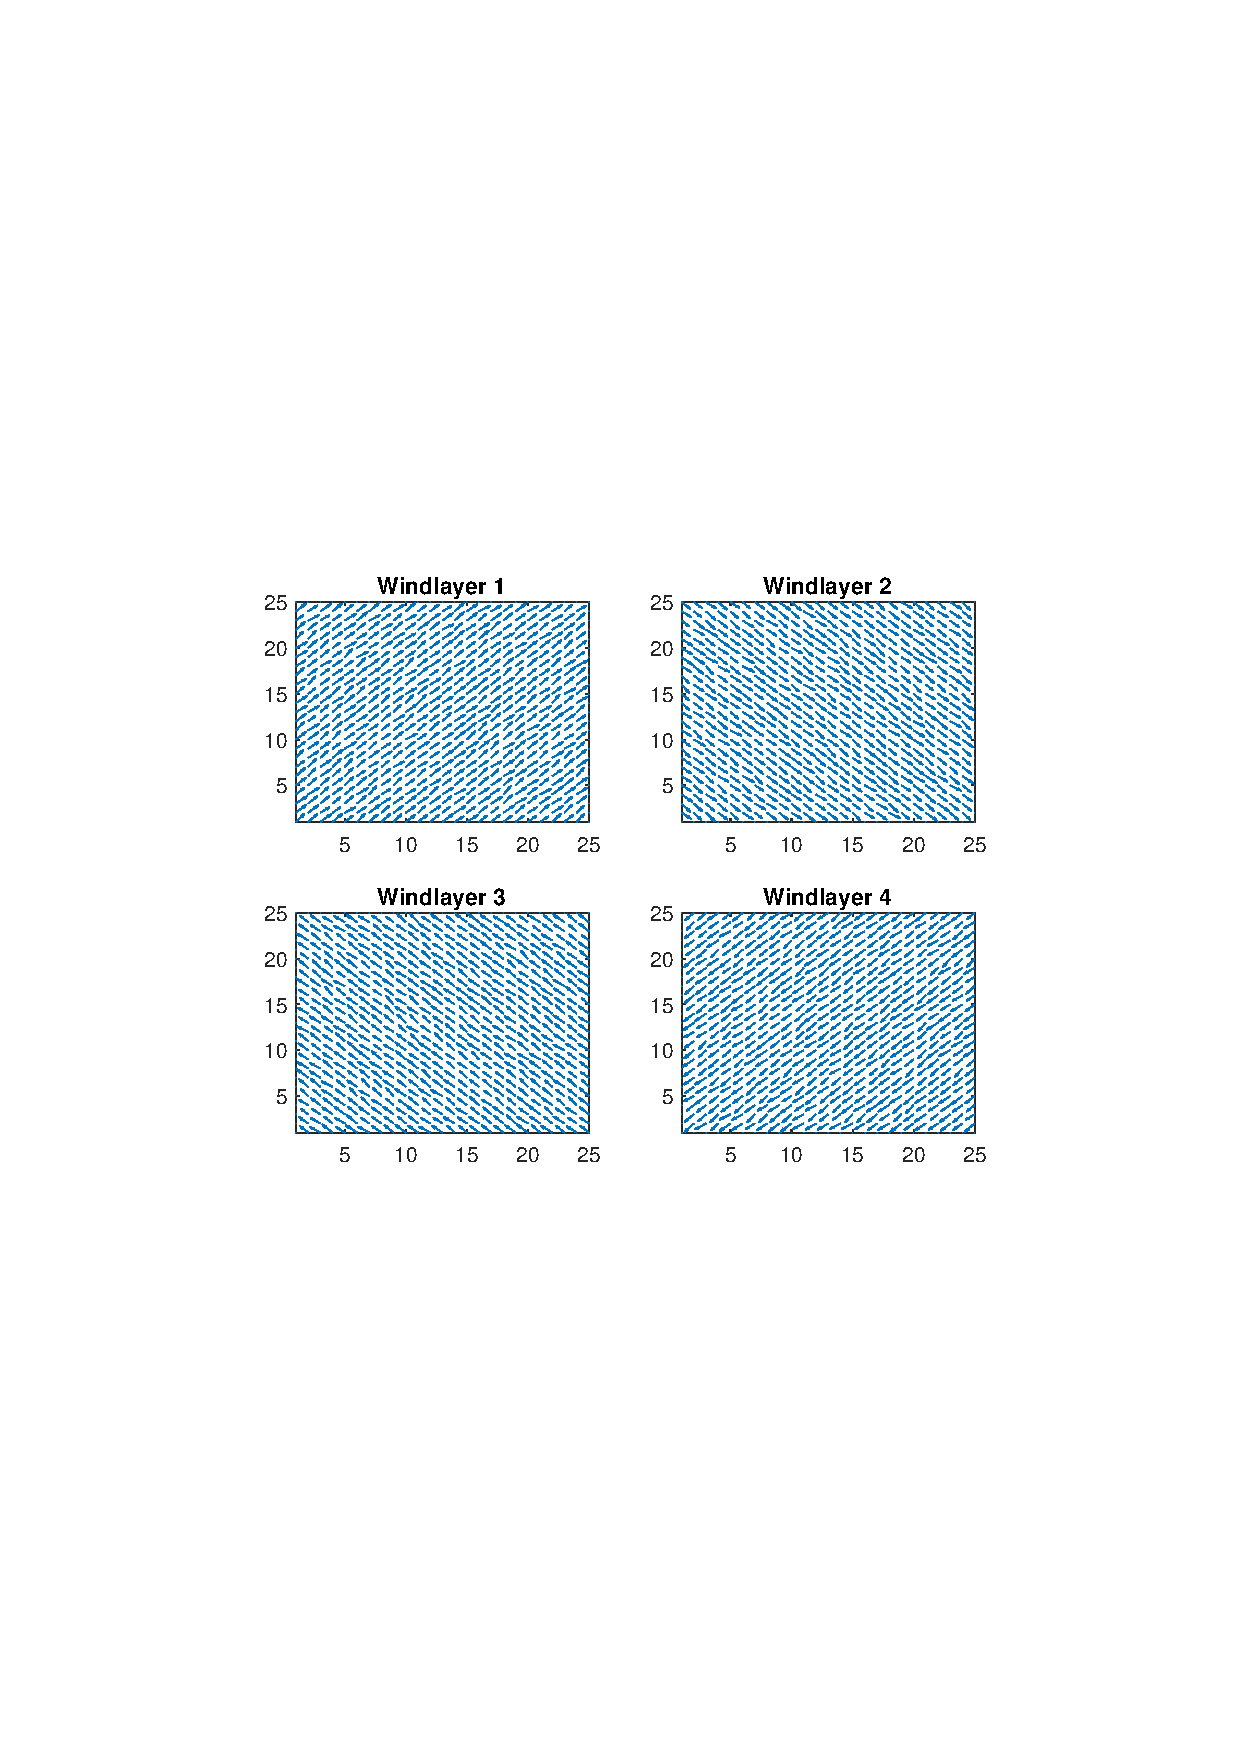
\includegraphics[width=\textwidth, trim={4cm 10cm 4cm 9cm},clip]{graphics/WindLayers.pdf}
\label{fig:windLayers}
\caption{Wind Layers}
\end{figure}


The stratosphere in the model is a collection of four layers, each with its own collection of wind vectors. The general direction of each is the same throughout the plane, but each vector has a deviation of about 10\% to make the behaviour realistic and give the control algorithms more directions to choose from. Each of the four layers have their own general direction, pointed towards one corner of the grid. This is done to increase variety of wind directions and possibilities to choose from. The average speed of the jet streams in the stratosphere is about miles an hour, or approximately 45 meters per second \citep{Roginsky1999}, which is used as a default size for the wind vectors. Figure \ref{fig:windLayers} shows an example of generated mock data set.




\subsection{Simulation and Parameters}\label{theModel_snp}
The model is the structure and relationship between all objects. It is modifiable in some ways to be able to measure and compare performance of different algorithms. The parameters that should be adjusted before simulation are the following:

\begin{description}
\item[WORLD\_SIZE:] The integer dimension of the grid that represents the earth. This number greatly affects the run time of the model as well as accuracy. 
\item[NUMBER\_OF\_BALLOONS:] The number of balloons in the model. This variable is usually set to the number of cells in the earth grid, i.e WORLD\_SIZE$^2$.This means that best case scenario the coverage is 100\% and all the balloons are perfectly spread.
\item[VERTICAL\_SPEED:] The speed of the balloon in directions up and down. This number will be added/subtracted from the balloon's altitude each step, until its motion in that direction is stopped.
\item[NUMBER\_OF\_STEPS:] How many steps the simulation should run. This number should be as big as possible to properly model the behaviour of the ecosystem. 
\item[NUMBER\_OF\_CURRENTS:] The number of wind layers, or wind currents, in the system. The more layers there is to choose from the more accurate direction the balloon should be able to choose from.
\item[MIN/MAX\_ALTITUDE:] Numbers used to divide the layers. The total distance between MIN and MAX is divided equally between all the layers in the model. This is used to determine whether a balloon has reached a new wind layer. The units are abstract but should be taken into consideration when choosing vertical speed. The vertical speed corresponds to the units in this MIN/MAX scale.
\end{description}

The model and simulation go hand in hand. When all objects have been created and configured, the simulation is run. 

The simulation moves all balloons according to the established stratosphere. Each step of the simulation the following process is as follows:

\begin{enumerate}
    \item Apply decisions: All balloons decide, using the control algorithm, whether they should start moving up or down or stay in the current altitude. 
    \item Apply currents: When the decision has been made, all the balloons are moved according to the wind layer they are currently located in. Furthermore they are moved up or down according to the model parameter for vertical speed. 
    \item Update statistics: The statistics of the simulation are gathered on the fly so after each iteration the data is re-evaluated and stored for further analysis.
\end{enumerate}



\subsubsection{Range}\label{theModel_numBal}
A fairly scientific method was used to determine a reasonable value for the range parameter. The following steps were taken to compute a reasonable value for the range: 

\begin{enumerate}
    \item What if the coverage was a square? Assuming a system with $n$ balloons, what is the size of each square patch?
    \item What is the size of the larges square patch that one circle can cover?.
    \item Infer answer from 1 and 2.
\end{enumerate}

The notations in the calculations map with the model parameters as stated here:

\begin{align}
    x &= \text{WORLD\_SIZE}\notag \\ 
    r &= \text{RANGE}\notag \\
    n &= \text{NUMBER\_OF\_BALLOONS} \notag \\
    a &= \text{Distance from circle center to edge of inner square} \notag \\
    A &=\text{Area of inner square of a circle} \notag \\
\end{align}

The world is a grid with area 
\begin{align}
S=x^2 \notag
\end{align}

The number of balloons is $n$ so each one is responsible for covering an area of size $\frac{x^2}{n}$. The distance from the center of a circle to the edge of its inner square is

\begin{align} 
a^2 + a^2 &= r^2 \notag \\
a &= \sqrt{\frac{r^2}{2}} \notag
\end{align}

but that means that the are of the inner square is

\begin{align}
A &= \frac{r^2}{2}
\end{align}
The goal was to fill the area $S$ but that means
\begin{align}
A &= S\notag \\
\iff \frac{r^2}{2} &= \frac{x^2}{n}\notag \\
\iff r &= \sqrt{\frac{2}{n}}\cdot x \notag \\
\iff RANGE &= \sqrt{2} \cdot \frac{WORLD\_SIZE}{\sqrt{NUMBER\_OF\_BALLOONS}} \notag
\end{align}
\begin{figure}[H]
    \centering
    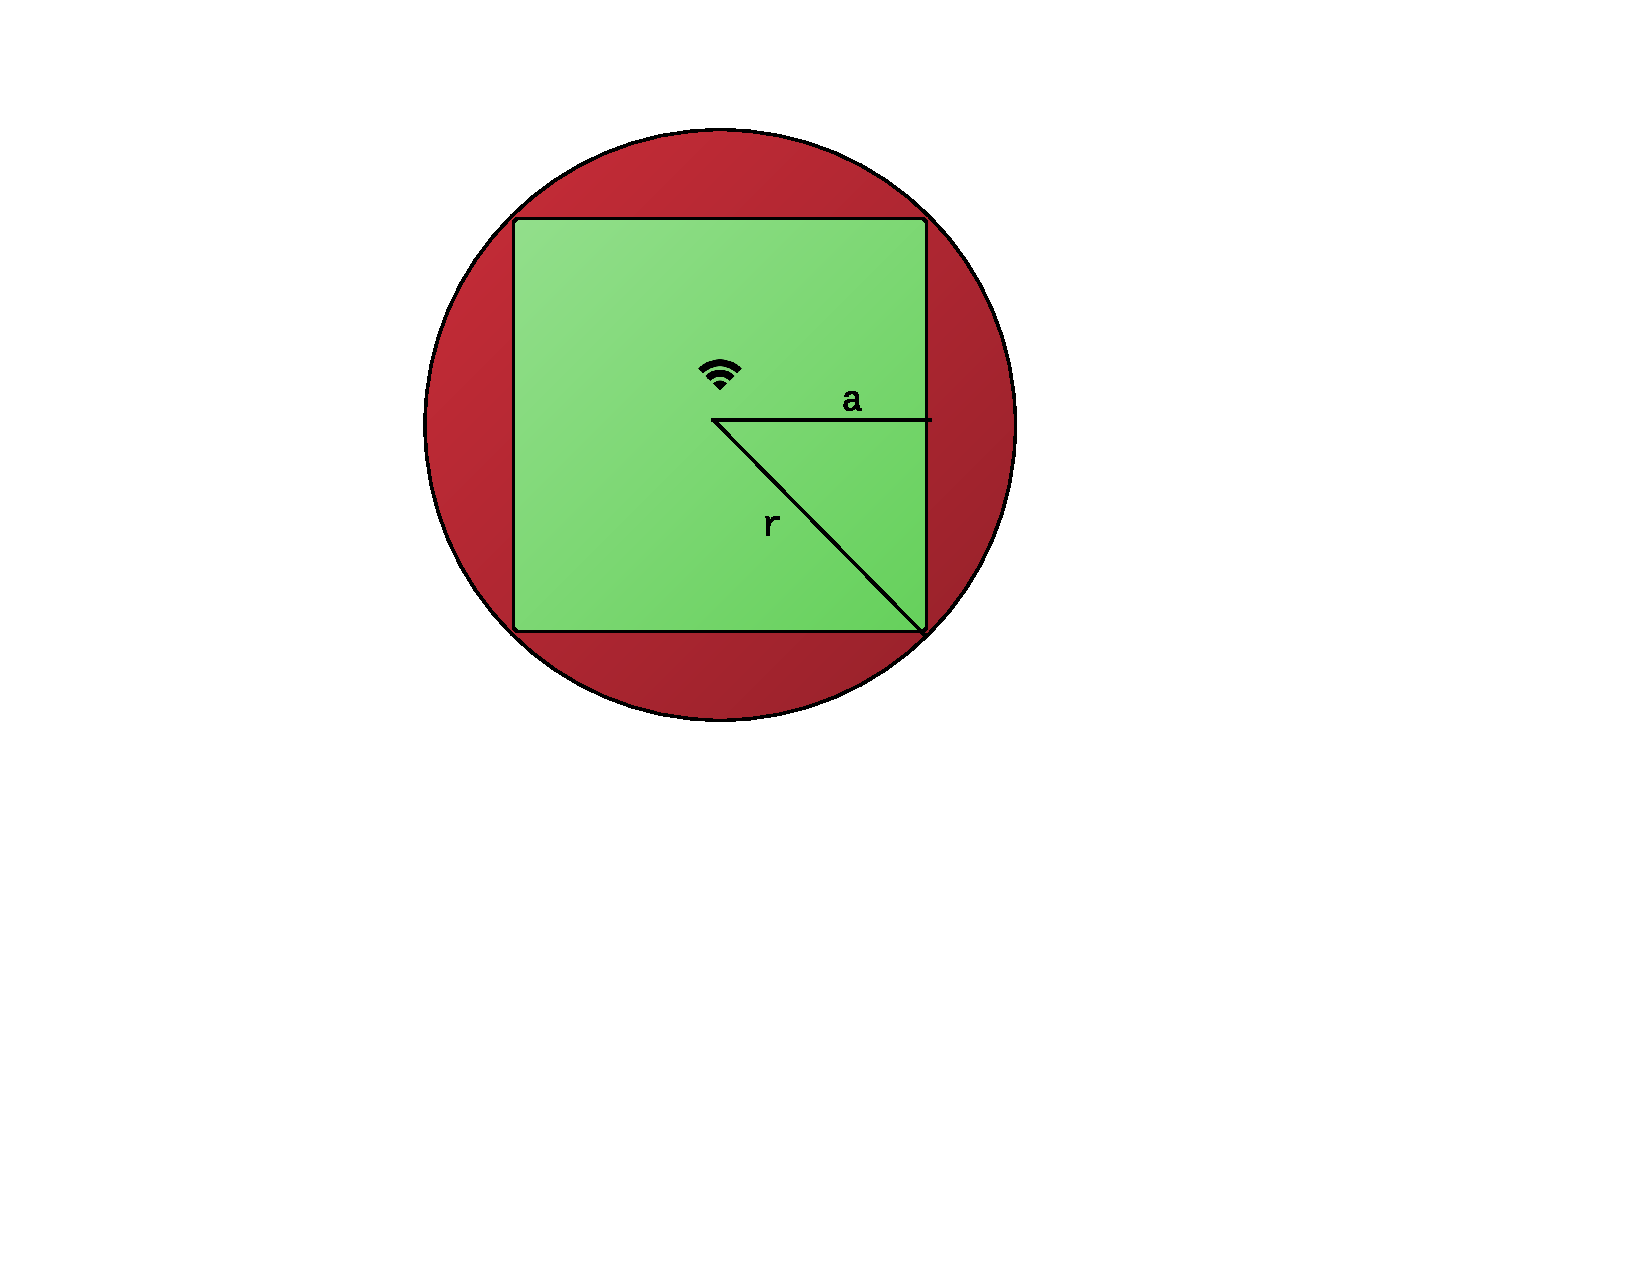
\includegraphics[scale = 0.5,trim=3cm 8cm 6cm 2cm, clip]{graphics/innersquare.pdf}
    \caption{Variables used for calculation of inner square}
    \label{fig:innersquare}
\end{figure}

Range is of course rounded to the next whole integer as the world is represented with an integer grid. But why programming this dependency between the model parameters range, world size and number of balloons? This model is an abstract version of the world and void of any units for length or size so controlling the ratio between the range versus the size of the grid is meaningless. This choice of range will clearly cover more than the actual area as displayed in figure \ref{fig:innersquare} but this is as good of a starting point as any. Modifying and exploring the effect of a smaller or larger range is of course possible and straight forward.

\subsection{Assumptions}
The assumption is made that the grid is fine grained and corresponds to a surface on earth. Each cell in the grid has a boolean and 

    $grid[x][y] == true$ for $x,y\in [0;\text{WORLD\_SIZE}]$
    
would represent a surface with lossless internet connection on every point. Each balloon occupies exactly one point in the grid but supplies coverage to the neighbouring area. The size of that area is controlled by the parameter RANGE. This is better displayed in figure \ref{fig:gridAssupmtions}.
\begin{figure}[H]
    \centering
    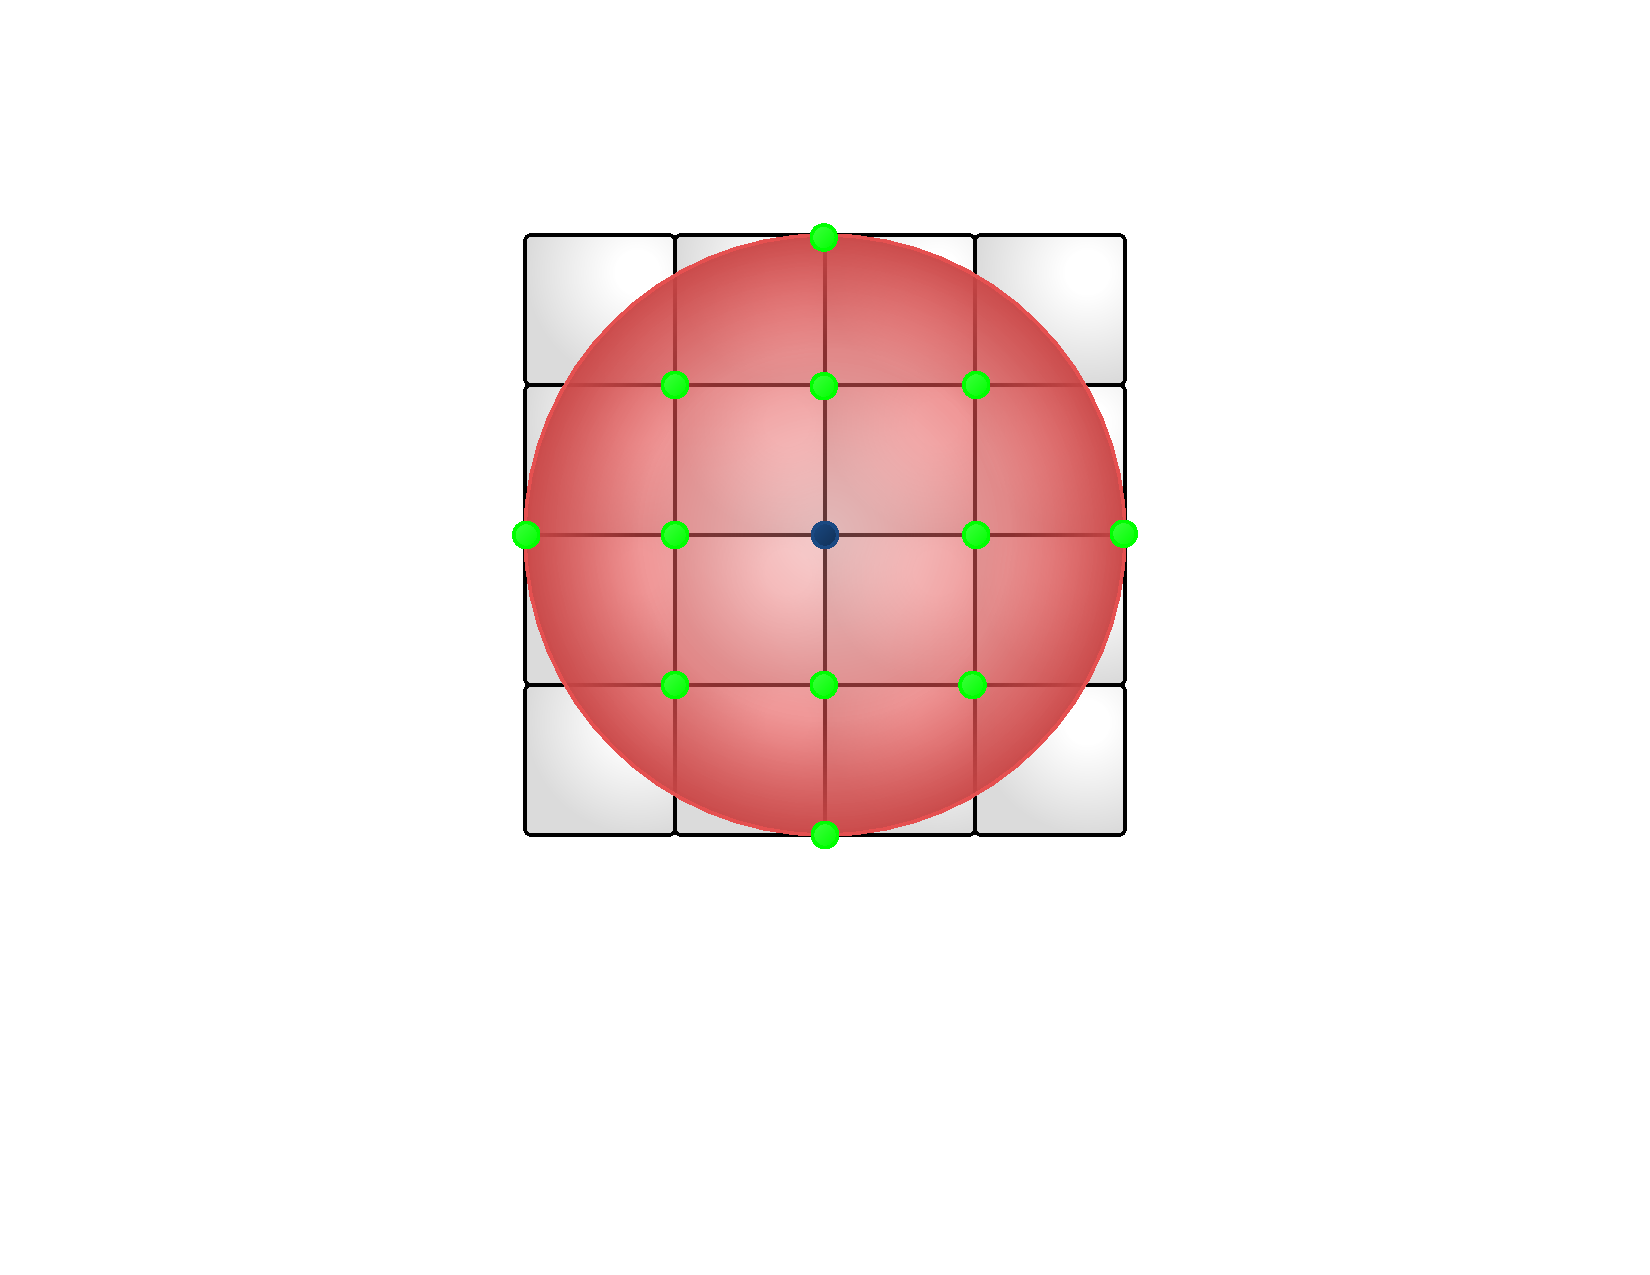
\includegraphics[width=\textwidth, trim=4cm 6cm 4cm 3cm, clip]{graphics/coverage.pdf}
    \caption{The figure displays the coverage in a 5x5 grid with a balloon at (2,2) and RANGE=2}
    \label{fig:gridAssupmtions}
\end{figure}
The actual placement of each balloon in regards to coverage on earth is somewhat irrelevant for this model, since the goal is to distribute the balloons evenly and keep them moving in an organized fashion, i.e keep each cell in grid above and close to 1. The grid of balloons is an abstract measurement of the distribution of the balloons and is sufficiently good tool to measure the quality of any control algorithm. 

The movement of a balloon in a grid is similar to the old Nintendo games. 

\begin{figure}[H]
    \centering
    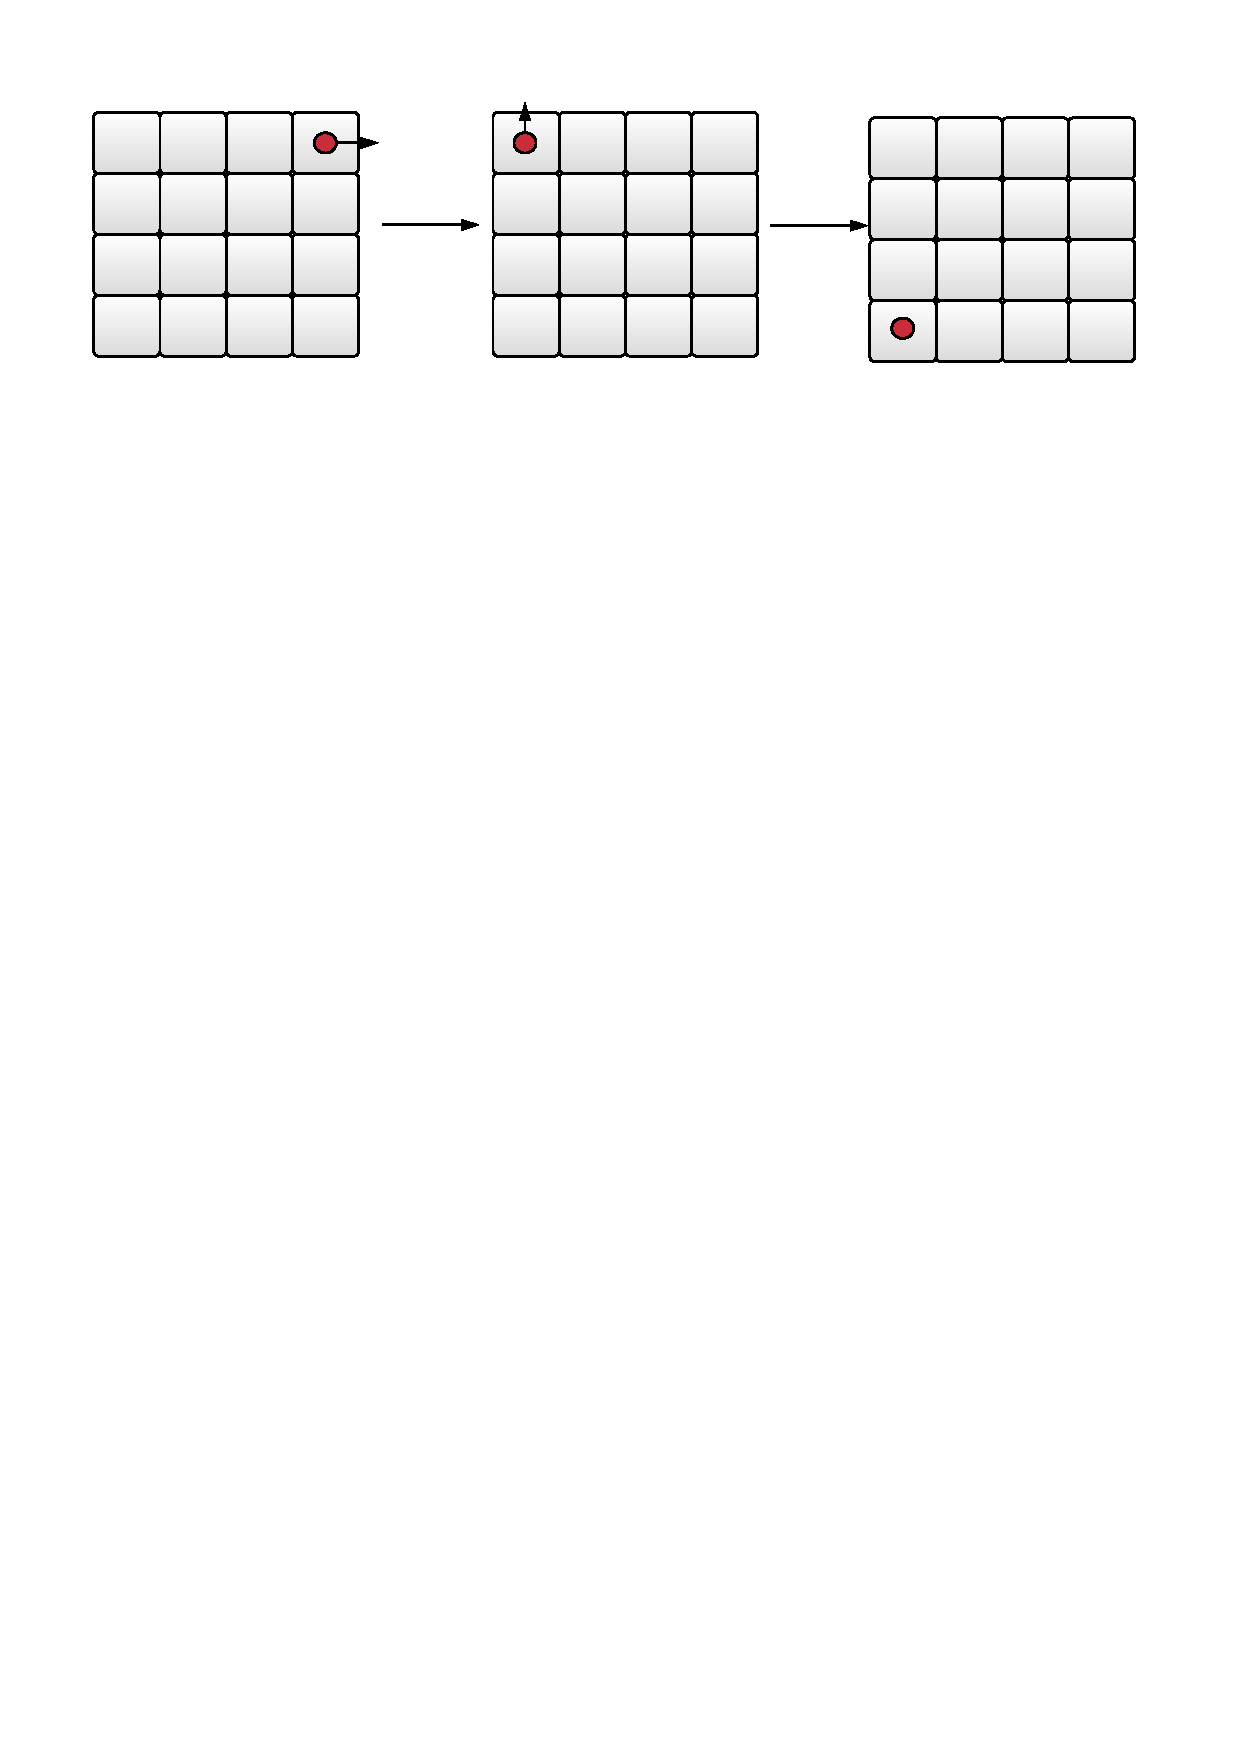
\includegraphics[width=\textwidth, trim=1cm 22cm 1cm 1cm, clip]{graphics/borderBehaviour.pdf}
    \caption{Border Behaviour}
    \label{fig:bb}
\end{figure}

When a balloon exits the grid it appears on the opposite site. This is done as a rudimentary attempt to resemble the behaviour of an object in a spherical grid when flattened out. 

In the model the balloons are a point in a grid, without a mass or volume. Also, the balloons do not move to a different spot in a continuous motion but are teleported between places. Removed from point A, and spawned at a point B. Multiple balloons are allowed to occupy the same space without any conflicts or implications. This is a simplification of the real life problem, but does not have to be included in the model as the odds of a crash are trivial when the size of the space the balloons occupy are taken into consideration. The model is however constructed so that removing this assumption would be easy. With the \textit{removeBalloon()} function the implication of a crash is easily implemented.

The current lifetime of a balloon is a fixed number in this model, which is an unlikely event in the real life problem. The balloons can however still not hover forever so this model parameter was necessary. The balloon is removed from the grid at the point where it was located when it reached is maximum age. This is convenient when modelling, but maybe not in the real life problem, since the balloon could be hovering over the sea, or a city, when it reaches its limit. The assumption is made that the balloon can be safely landed at every point in the grid. 

All new balloons are launched from the same place, at cell (0,0) in the grid. More launching places could easily be implemented by modifying the createBalloon() function or by using the override function createBalloon(int x, int y) which lets the user choose a specific location to which the new instance of the Balloon class should be created.

The weather data and the vertical movement of the balloons has been simplified greatly. The mock data created has been created really conveniently to give the balloons as many directions to choose from as possible. This is not always the case in the stratosphere. Furthermore, the division between different wind layers is not as clear as portrayed in this model. The data is however realistic enough to give weight to the model and display a lifelike behaviour of the balloons to some extent. The balloons move between two points in every step of the simulation, whether it is with one layer or another, and that behaviour is sufficient at this stage.

The assumption is made that the coverage on earth does not depend on the altitude of a balloon. This is a simplification since the signal strength from a balloon differs from altitude to altitude. This is overlooked in this model but can easily be implemented in an updated version, since this is only a matter of calculations and usage of units and measurements that already are available in this model. 





\subsection{Measurements and output}
The collection of data in the model is twofold. First there is static data which is collected before and after the simulation. Those measurements include the parameters of the model as well as: 

\begin{description}
    \item[droppedConnections: ] The number of times a balloon leaves a spot and leaves it uncovered. That would mean that the connection would drop in that area until another balloon would fly over.
    \item[accumulatedCoverage: ] The accumulated coverage of the simulation divided by the number of steps. This gives a concrete value for the quality of the control algorithm.
    \item[run time: ]The time it took to run the simulation.
\end{description}

These three results, as well as the values for the parameters, are appended to a file called simulation\_results.txt which is a log file for the model. 

The current coverage at step $t$ is output to a text file which is named after the algorithm used in that simulation, e.g. simulation\_coverage\_alg1.txt. This file is overwritten every simulation and has the following format.
\begin{table}[]
\centering
\begin{tabular}{l|l}
Step number & Current Coverage
\end{tabular}
\caption{simulation\_coverage file format}
\end{table}

\section{Design}
\subsection{The Model}


This model was designed following the \textit{General Responsibility Assignment Software Patterns} (GRASP). The GRASP design principles provide guidelines for object-oriented software design and are well suited for a project such as this. The main focus of the principles, like the name states, is assigning responsibilities to the appropriate objects in the model. The basic roles in GRASP can be divided into \textit{knowing} and \textit{doing}. The design of the loon model is simple so the division was straight forward:
\begin{itemize}
\item[BALLOON:]
    \subitem Knows: A balloon object knows its own location, altitude and in which wind layer it is currently located.
    \subitem Does: A balloon object can move with the wind. It gets the wind vectors from the wind layer in which it is located. 

\item[WIND LAYER:]

    \subitem Knows: A wind layer object knows its own identification number, as well as the wind vector at any given place in the grid.
    \subitem Does: A wind layer does nothing but provide access to its data.

\item[WORLD:]

    \subitem Knows: The world know about the status of the simulation and how many steps have been taken. It collects statistical data about the grid in which the balloons hover. 
    \subitem Does: The world has access to all balloons and wind layers and is the controller of the simulation. The world initiates all decisions and movements of every balloon. 

\end{itemize}

The Balloon and WindLayer are expert classes while World is a controller class in this model. The algorithms developed during this project will be centralized, i.e controlled by an entity with knowledge of the entire system and access to all objects. This limits the balloons' responsibility to simply stay in the air, take commands and supply Internet coverage.

\begin{figure}[H]
    \centering
    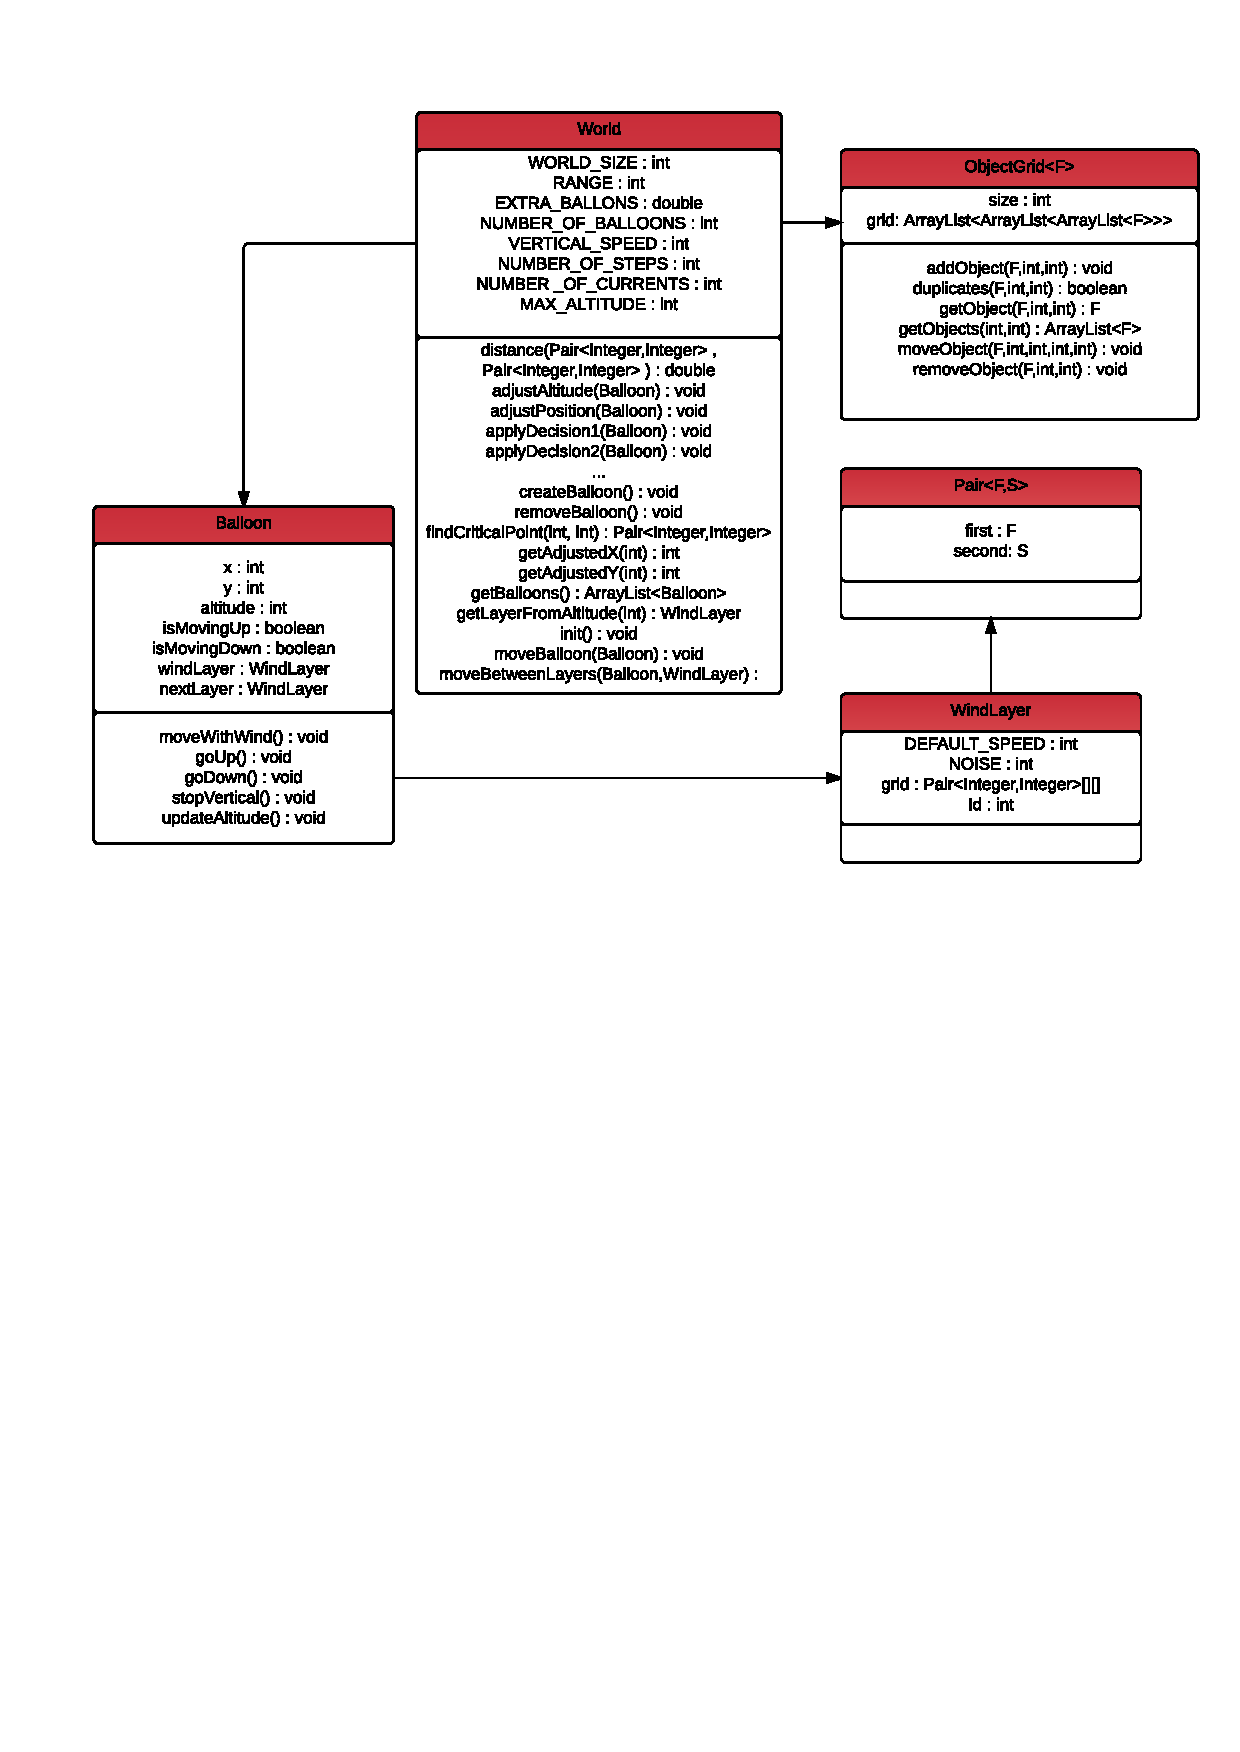
\includegraphics[width=\textwidth, trim= 1cm 14cm 0cm 0cm, clip]{graphics/classDiagram.pdf}
    \caption{Class Diagram}
    \label{fig:class_diagram}
\end{figure}


\begin{figure}[H]
    \centering
    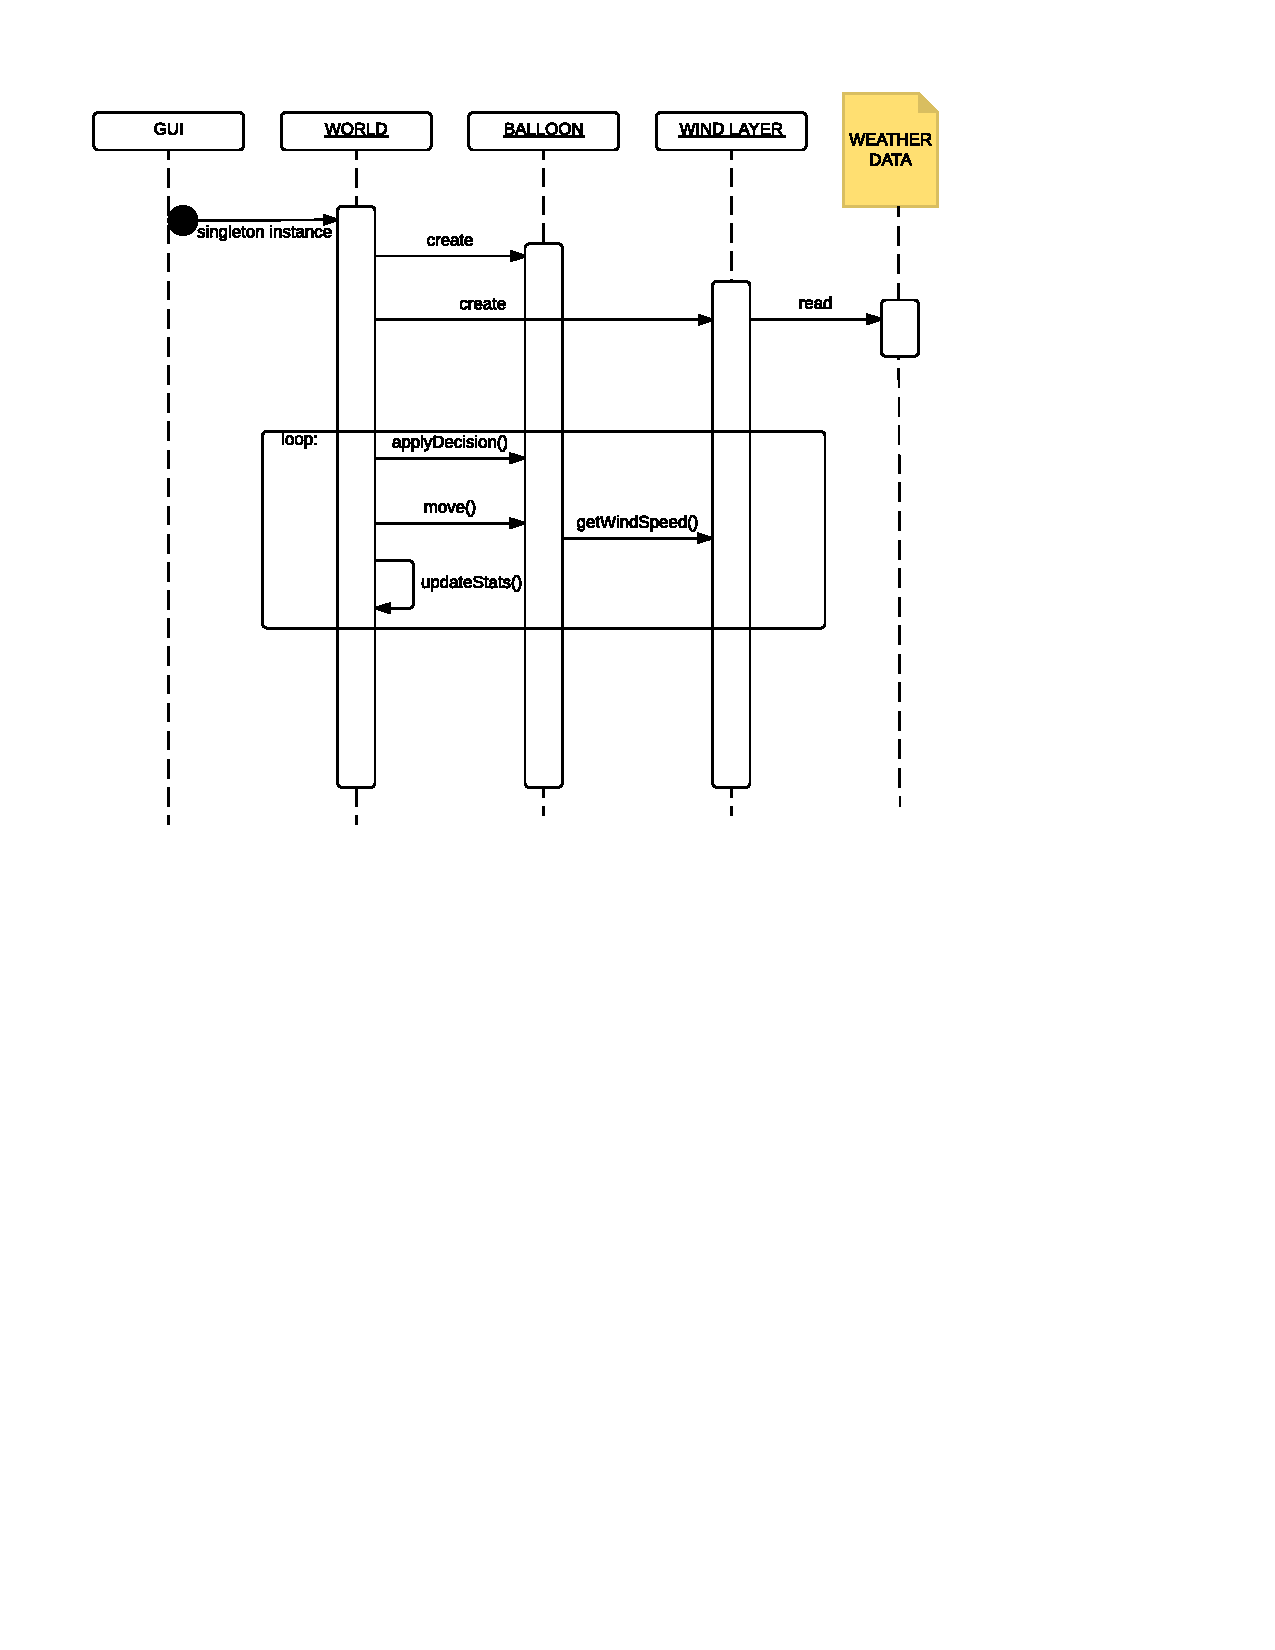
\includegraphics[width=\textwidth, trim= 1cm 12cm 4cm 1cm, clip]{graphics/sequenceDiagram.pdf}
    \caption{Simplified Sequence Diagram}
    \label{fig:seq_diagram}
\end{figure}


\subsection{GUI}
Two user interfaces were developed for the model. The first one, named \textit{TextGUI}, a pure textual output displaying all the statistical data for the simulation as well as generating text files with the sequence of coverage data during the run. This was used comprehensively to analyze and compare the performance of different algorithms. 

The second one, named \textit{MainWindow}, provided graphical representation of the balloons at each step. The design was very rudimentary and was developed purely for debugging purposes at early stages of the project. Seeing the initial movements of the heard of balloons gives a clear image of the behaviour of the model and whether it is working properly or not. The simulation window gives the user an opportunity to take a single step, or up to 200 steps at at time, using the slider object.


\begin{figure}[H]
    \centering
    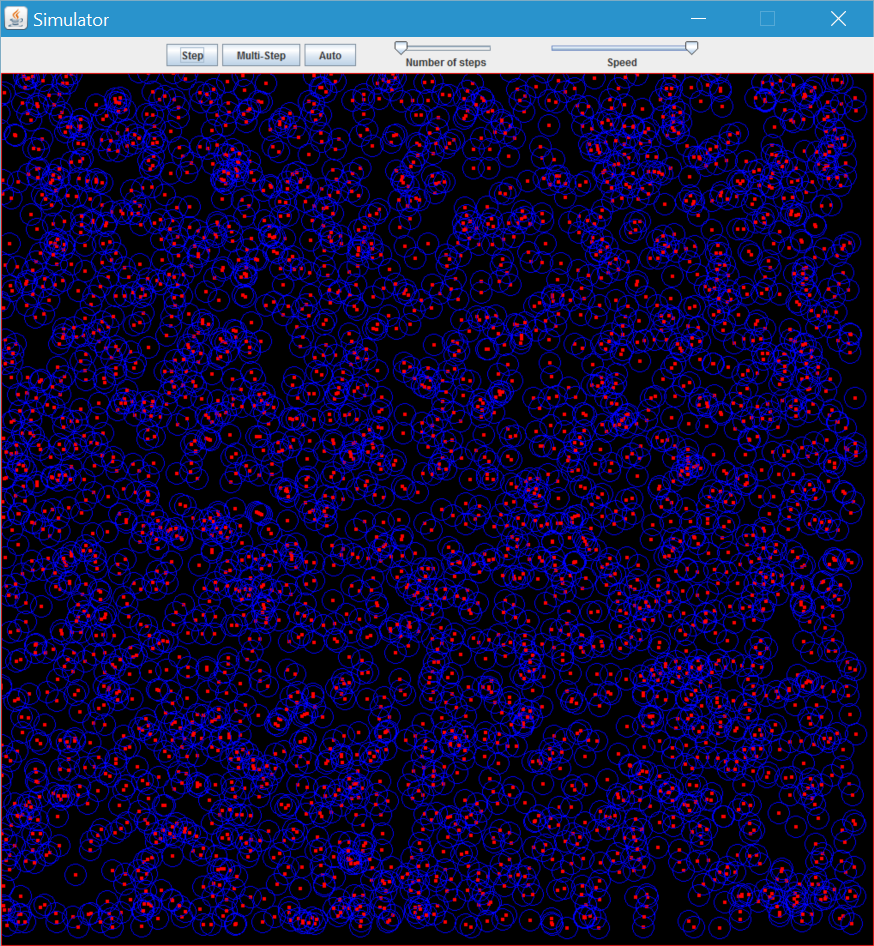
\includegraphics[width=0.7\textwidth]{graphics/MainWindow.png}
\caption{Simulator}
\label{fig:mainwindow}
\end{figure}

The speed of the simulation can be controlled with another slider object. This second interface is not bound to the model parameter NUMBER\_OF\_STEPS so it will run until stopped. This is useful to see how an algorithm works during long simulations. In this project a visual representation is often the fastest measure of quality of an algorithm. 

\section{Implementation}
The programming language of choice for this project was JAVA. That was well suitable for an object oriented problem such as this. Eclipse was used as an IDE not only because of familiarity, but also due to all the handy refactoring tools that come built in to the environment. This is helpful when the code starts to look complicated, to be easily able to extract lines of code and store it within a private helper function. The toolkits SWING and AWT were used for the development of the GUI.

The project was stored on GitHub\footnote{www.github.com/karithrastarson} and is accessible to everyone. The process was iterative where a running version of the model was ready early, and then built upon for the duration of the period.
\subsection{Balloon}

The balloon class is an expert for the balloon. The following attributes are used to describe the object:
\begin{description}
	\item[int x]: X coordinates in the plane
	\item[int y]: Y coordinates in the plane
	\item[int altitude]: the altitude is used to determine wind layer
		\item[int age]: the number of steps this balloon object has taken.
	\item[boolean isMovingUp]: Used to determine whether this balloon is currently moving up.
	\item[boolean isMovingDown]:Used to determine whether this balloon is currently moving down.
	\item[WindLayer windLayer]: The current wind layer this balloon is located in.
	\item[WindLayer nextLayer]: Used to determine whether where this balloon is headed.
\end{description}

The balloon's main function and responsibility to the model is to move with the wind. This is done with the public function moveWithWind(). The balloon retrieves a wind vector from its current wind layer and adds the x and y components of that vector to its own current location in the grid. The new coordinates are then adjusted by the model, according to the border behaviour as described earlier. The adjustment is made as follows:

\begin{algorithm}[H]
\If{new x $\geq $ WORLD\_SIZE}{set x = x-WORLD\_SIZE}
\If{new x < 0}{set x = x+WORLD\_SIZE}

repeat for Y.\\
\end{algorithm}

The rest of the functions in the Balloon class are classic getters and setters, as well as a toString() and equals() functions.

\subsection{WindLayer}
The WindLayer class is an expert of weather data. Its main attribute is a grid of size equal to the WORLD\_SIZE global variable. The default constructor of the class takes two variables; an ID and the size of the world in which it will be. From that information the constructor takes care of generating mock data for the wind layer.

Two global variables are used to adjust the mock data:
\begin{itemize}
    \item DEFAULT\_SPEED = 45
    \item NOISE = 5
\end{itemize}

Algorithm \ref{alg:mockdata} displays how the mock data is generated. This model uses 4 layers and the constructor uses the ID to determine the general direction. The default speed variable is set to one of the four corners of the plane, based on the ID. Then a random number is generated on the scale from zero to the predefined max noise. Then a random boolean variable determines whether that random number should be added or subtracted from the x direction of the wind vector. Same routine is performed for the y direction. 

\begin{algorithm}[H]

\For {i from 0 to WORLD\_SIZE}{ 
    \For{j from 0 to WORLD\_SIZE}{


\If{Id=0}{x=DEFAULT\_SPEED and y=DEFAULT\_SPEED}


\If{Id=1}{x=DEFAULT\_SPEED and y=-DEFAULT\_SPEED}


\If{Id=2}{x=-DEFAULT\_SPEED and y=DEFAULT\_SPEED}


\If{Id=3}{-DEFAULT\_SPEED and y=-DEFAULT\_SPEED}

div = random number from 0 to NOISE

signX = random boolean

\If{signX}{x + div}
\Else{x - div}\endIf

div = random number from 0 to NOISE

signY = random boolean

\If{signY}{y + div}
\Else{y - div}\endIf

wind[i][j] = wind vector(x,y)
}
\EndFor}
\EndFor
\caption{Pseudocode for generating mock data}
\label{alg:mockdata}
\end{algorithm}


\subsection{Pair}
This class was created when a short survey on the Internet showed that JAVA was not equipped with a convenient generic container class that would store pairs, or tuples. It was easier to implement one from scratch. This class is really simple: it carries two variables of generic types T and R. Then the class is equipped with getters and setters. 

This class was created to contain the wind vectors. Each wind layer has a grid of Pairs. So a pair at coordinates x and y in a grid in the layer tells the wind speed and direction at that particular point.

\subsection{ObjectGrid}
No Java library had a suitable container for this project. The object that this project demanded was a two dimensional grid of a fixed size that could store zero or more objects in each cell. A generic class was implemented, but it was then utilized with Balloon objects in this particular project. This makes it easier to access a particular balloon object based on its coordinates.

The main container of the class looks complex but is in fact really simple. The class has the following attributes:

\begin{lstlisting}
    private ArrayList<ArrayList<ArrayList<F>>> grid;
    private int size;
\end{lstlisting}

The outer two array lists are initialized in the constructor, and a grid of empty array lists created. This grid has the dimensions size x size. Each cell in the grid holds an array list of a generic type that can be populated and modified easily. To find the number of balloons occupying a certain spot, the size of the array list at the corresponding cell in the grid is generated and returned.

\subsection{World}
The world is the controller of the model and contains all the balloons, wind layers and the control algorithms. The class contains a lot of attributes who's sole purpose is debugging and printing to to create graphs. Those attributes will be left out of this documentation. 

The World class has the attributes listed in section \ref{theModel_snp}. The class has two main containers that make up the model:

\begin{lstlisting}
	private ArrayList<WindLayer> stratosphere;
	private ArrayList<Balloon> balloons;

\end{lstlisting}

In addition, the class has three containers that support the decision making and the statistical overview of the simulation:
\begin{lstlisting}
	private ObjectGrid<Balloon> balloons_grid;
	private boolean[][] coverage;
	\end{lstlisting}
The ArrayList called \textit{stratosphere} holds all wind layers of the model in an order. The ArrayList called \textit{balloons} is a collection of all balloons created by the model. The boolean grid called coverage is updated in every step of the simulation with boolean values; true for covered and false for not covered. The ObjectGrid called balloons\_grid keeps track of the position of all balloons in the system.


\begin{algorithm}[H]
    Clear the grid.\\
    \ForAll{Balloon b in balloons}
    {center = Pair(b.getX(), b.getY())\\
        \For{int i = b.getX() - RANGE; i $<$ b.getX() + RANGE; i++}{
        \For{int j = b.getY() - RANGE; j $<$ b.getY() + RANGE; j++}{
        point = Pair(i,j)\\
        
        coverage[i][j] = inCircle(center, point)
        }
        }
    }
 \caption{Update Coverage}
 \label{alg:updateCoverage}
\end{algorithm}

The World class has a private function called updateCoverage() which is in charge of updating the boolean grid. This is described with algorithm \ref{alg:updateCoverage}. This function iterates through all the balloon in the system and inspects a rectangular area around the center of the balloon. This rectangle is visualized in figure \ref{fig:gridAssupmtions}. Each point in this area is passed through a function called inCircle, which applies the mathematical function for a circle to determine whether the point is within the coverage range or not. Either this points is within range or not. The sum of of all connected points is calculated and compared against the sum of the previous step. The difference in covered cells is interpreted as a dropped connection. If the connected cells er fewer than they were in the round before, that means that somebody has lost his Internet connection.

\begin{align}
    \left(x - a \right)^2 + \left( y - b \right)^2=r^2.\notag
\end{align}
where
\begin{align}\notag
     		x &= \text{x-coordinate}\\\notag
				y &= \text{y-coordinate}\\\notag
				a &= \text{x-coordinate of the center point}\\\notag
				b &= \text{y-coordinate of the center point}\\\notag
				r &= \text{radius (Range)}\notag
\end{align}


The constructor is short and only initializes the containers mentioned above without populating them. Then a more elaborate initialization function (called init(char c)) can be called with a character as an input, indicating which algorithm to use for the simulation. The \textit{init} function creates four wind layers and adds them to the stratosphere. Furthermore it outputs the windlayers to text files so they can be plotted and analyzed. The outcome is displayed in figure \ref{fig:windLayers}. 

One by one the balloons are created at placed at point (0,0) in the grid. Each step of the simulation adds on balloon and moves the rest. This will prevent the cell (0,0) from clogging on the first step.
The simluation is a repetition of the private function \textit{step()} and repeated as many times as the parameter of the model says. Each step is an execution of the following:

\begin{algorithm}[H]
\If{No. of balloons in system $<$ NUMBER\_OF\_BALLOONS}{createBalloon()}

\ForAll{balloons in system}{
applyDecision()
moveBalloon()
}

\ForAll{balloons in system}{
\If{Age of balloon $\geq$ LIFETIME}{removeBalloon()}
}

updateStatistics()
\end{algorithm}

The applyDecision() function is the actual control algorithm to which another section of this paper is dedicated. The moveBalloon() function is the thoughtful procedure of moving the balloon in the model and updating the appropriate containers. First the altitude is adjusted according to the vertical speed if the balloon is marked as moving up or down. Then a check is performed to see if the change in altitude affected the wind layer in which the balloon is. This is done with a function called \textit{getLayerFromAltitude} where each wind layer is assigned a certain space between the global variables that indicate the maximum and minimum altitude. The \textit{windLayer} attribute of the balloon is then updated and compared to the \textit{nextLayer} attribute to see if the vertical movement of the balloon should be stopped or not. 

When the balloon has been placed in the correct wind layer it can be moved around in the grid of balloons with the corresponding wind vector. The previous location as well as the new location of the balloons are updated in the grid to represent the actual movement. 



\section{Control Algorithms}
\subsection{Simulations}
The following values were used for the simulations unless otherwise stated:

\begin{table}[H]
\centering

\begin{tabular}{l|l}
World Size         & 200     \\ \hline
Lifetime           & 200 or LONG   \\\hline
Number of Balloons & 200 \\\hline
Range & 19 (computed) \\\hline
Communication Radius & 10 \\\hline
Vertical Speed     & 40      \\\hline
Number of Steps    & 1000  \\\hline
Number of Currents & 4       \\\hline
Max Altitude       & 400     \\\hline
Min Altitude       & 0 \hline      
\end{tabular}
\caption{Simulation Parameters}
\label{tbl_modelParameters}
\end{table}


\subsection{Algorithm 1}
The first algorithm is straightforward and rudimentary. Like the description of the model stated the simulation first checks if it can add balloons to the system. After doing so each balloon in the system uses the following logic to determine whether it should move or not:

\begin{algorithm}[H]
  \If{Multiple balloons same spot}{
 	\If{At bottom layer} 
 	{Go up}
 	\ElseIf{At top layer}  	
 	{Go Down}
 	\Else  	
 	{Choose direction at random}
 }
 \Else
 {Stay in current layer}
 \caption{Control Algorithm 1}
 \label{alg1}
\end{algorithm}

This algorithm has an obvious downside since as it contains an element of random, which is usually not helpful in a control algorithm. Nevertheless, it spreads the balloons thoroughly around the grid relatively fast. The control over the grid is however limited and this would not be a suitable solution if the end goal is to provide stable coverage.

This algorithm might however be utilized as a part of a larger more complex algorithm. At the beginner stages of the balloon's life cycle it could prove helpful to get the balloon out of that first wind layer and join the huddle.  

\subsection{Algorithm 2}
This algorithm is a step towards a more complex control algorithm. Some minor logic replaces the random generator in the previous solution. 

\begin{algorithm}[H]
  \If{Multiple balloons same spot}{
  Calculate projections\;
  
 	\If{optionUp < optionDown} 
 	{Go up}
 	\Else
 	{Go down}

 }
 \Else
 {Stay in current layer}
 \caption{Control Algorithm 2}
 \label{alg2}
\end{algorithm}

The balloon fetches the wind vectors from neighbouring wind layers and uses them to weigh its options. It computes the number of balloons occupying three different cells:
\begin{enumerate}
\item The cell to which the balloon's current wind layer will move it.
\item The cell to which the the wind layer above the balloon's current wind layer would move it.
\item The cell to which the the wind layer below the balloon's current wind layer would move it.
\end{enumerate}

The algorithm then determines which option has the cell with the lowest number of balloons and chooses that direction.
\begin{figure}
\centering
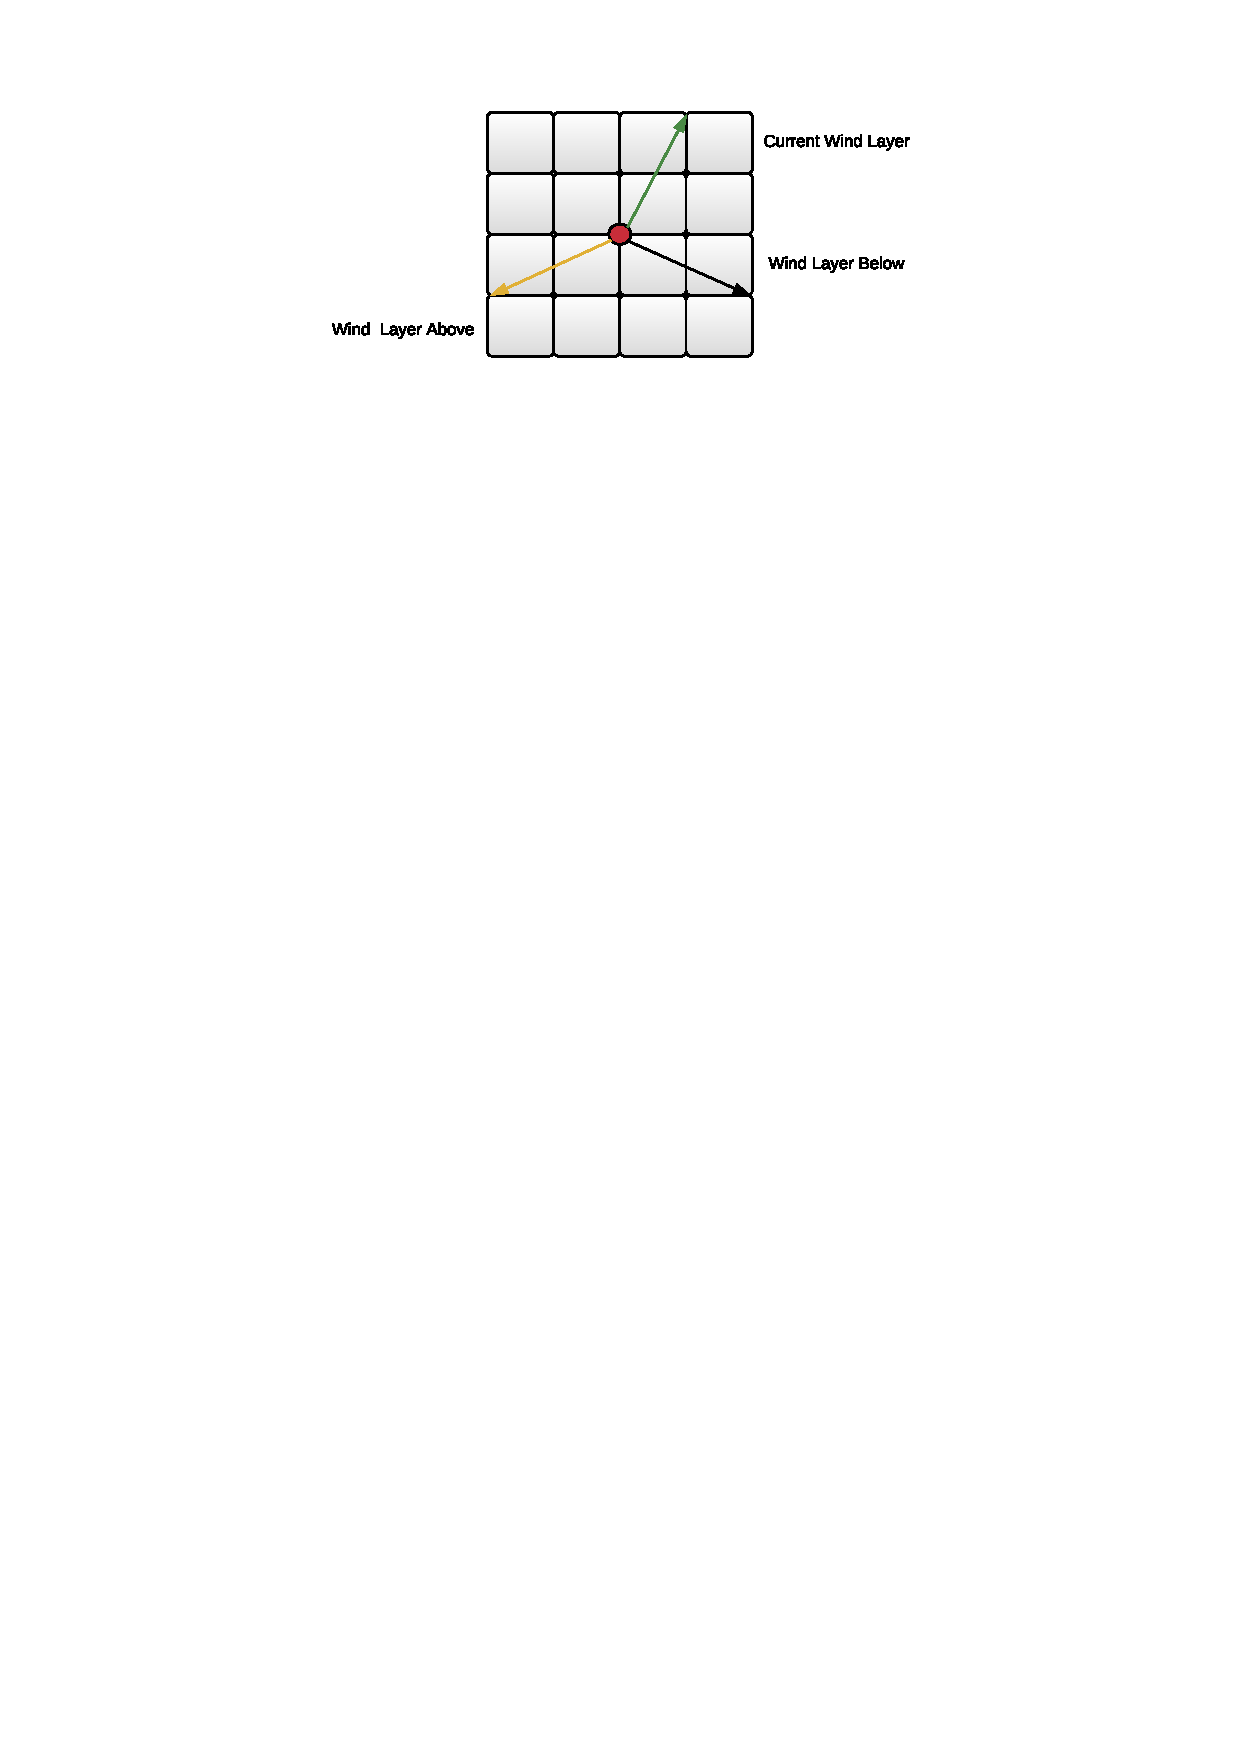
\includegraphics[width=0.8\textwidth,trim= 4cm 23cm 4cm 1cm,clip]{graphics/Projections.pdf}
\caption{Calculate projections}
\label{fig:projections}
\end{figure}

\begin{figure}
\centering
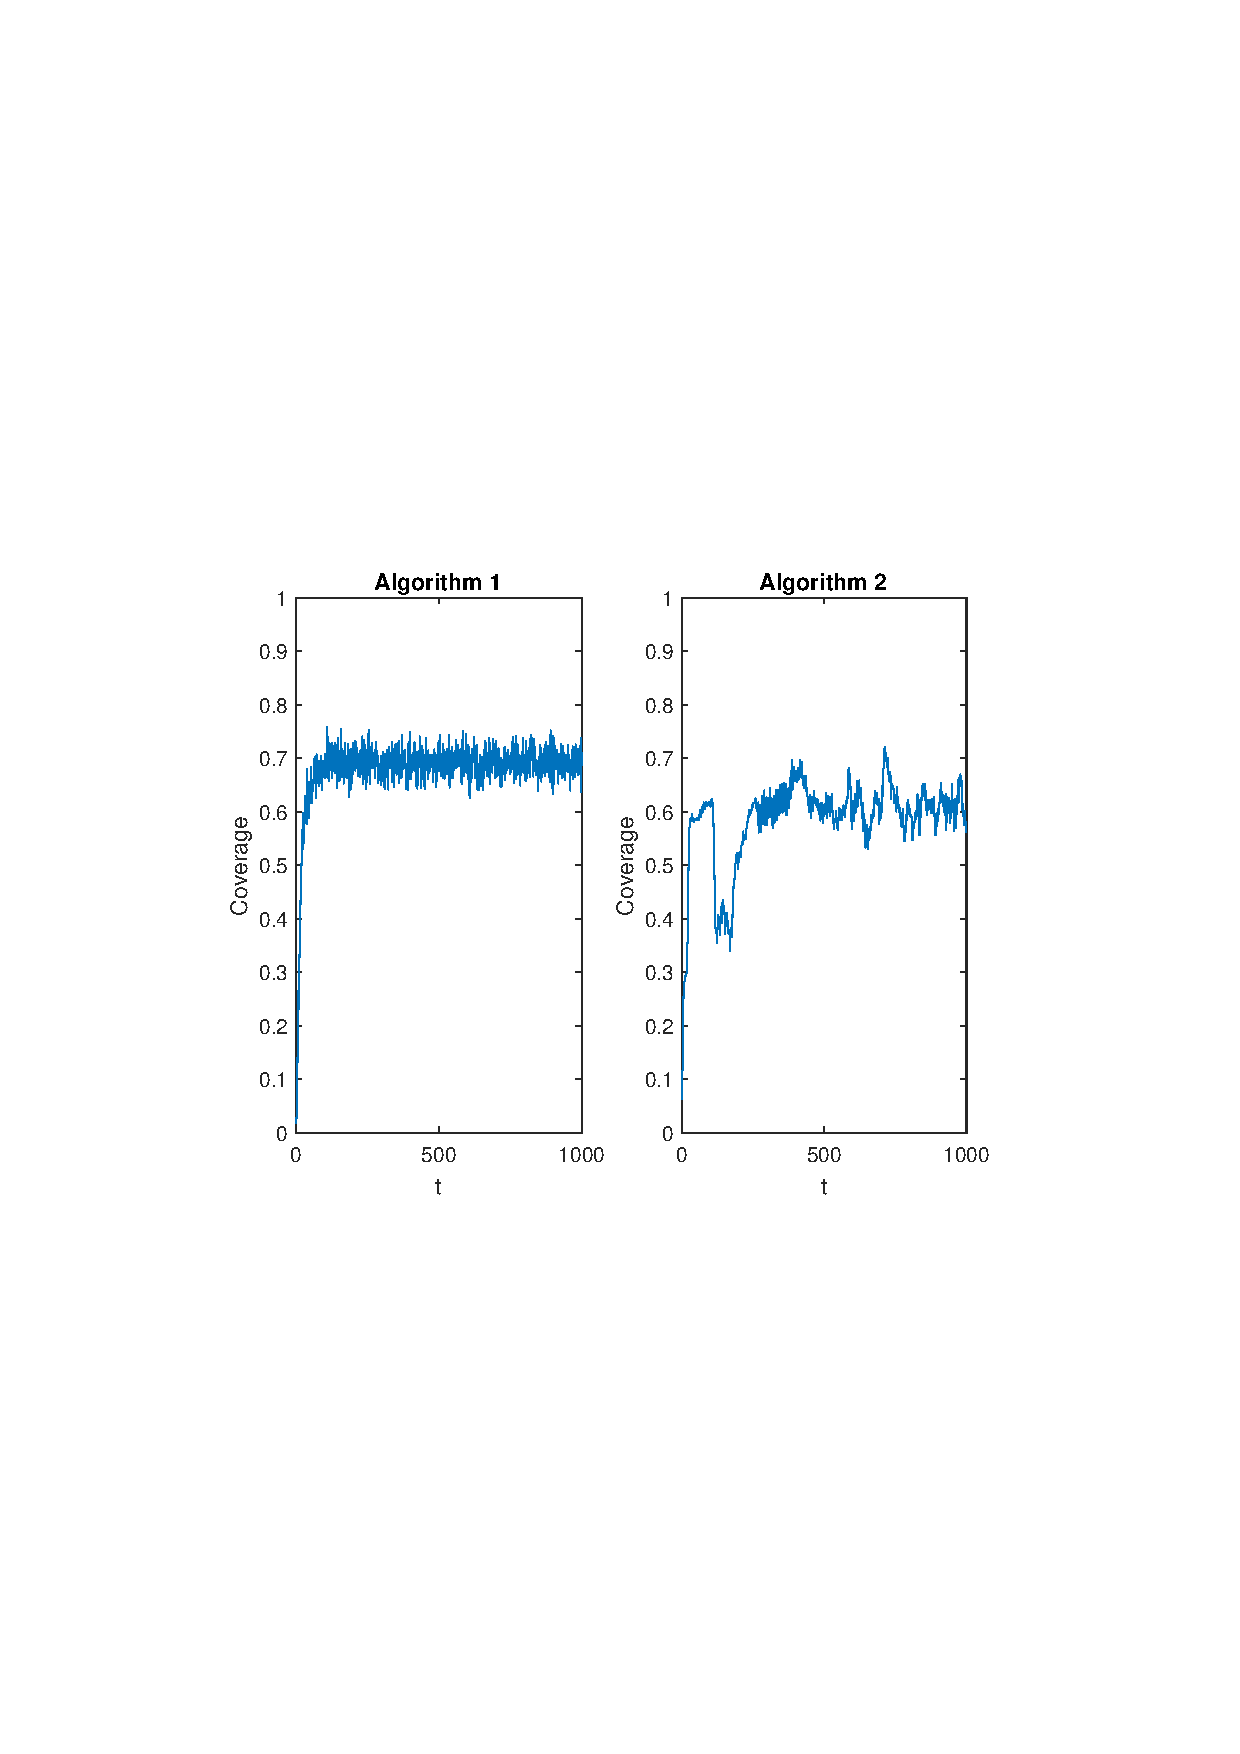
\includegraphics[scale=0.7, trim={3cm 10cm 4cm 9cm},clip]{graphics/coverage_alg1_vs_alg2_1000steps_LIFETIMELONG.pdf}
\caption{Algorithm 1 vs. Algorithm 2 in 1000 steps with an infinite lifetime of each balloon}
\label{fig:alg1vsalg2}
\end{figure}
It is interesting to see that Algorithm 1 outperforms Algorithm 2 when it comes to coverage and stability. Not only did Algorithm 1 reach higher coverage like Figure \ref{fig:alg1vsalg2} clearly shows but was also more stable. Multiple simulations were run and the each output graph was from Algorithm 1 was exactly the same while the graph for Algorithm 2 was changed with every each simulation. The figure of the comparison shows a typical output for both algorithms.

\begin{figure}
\centering
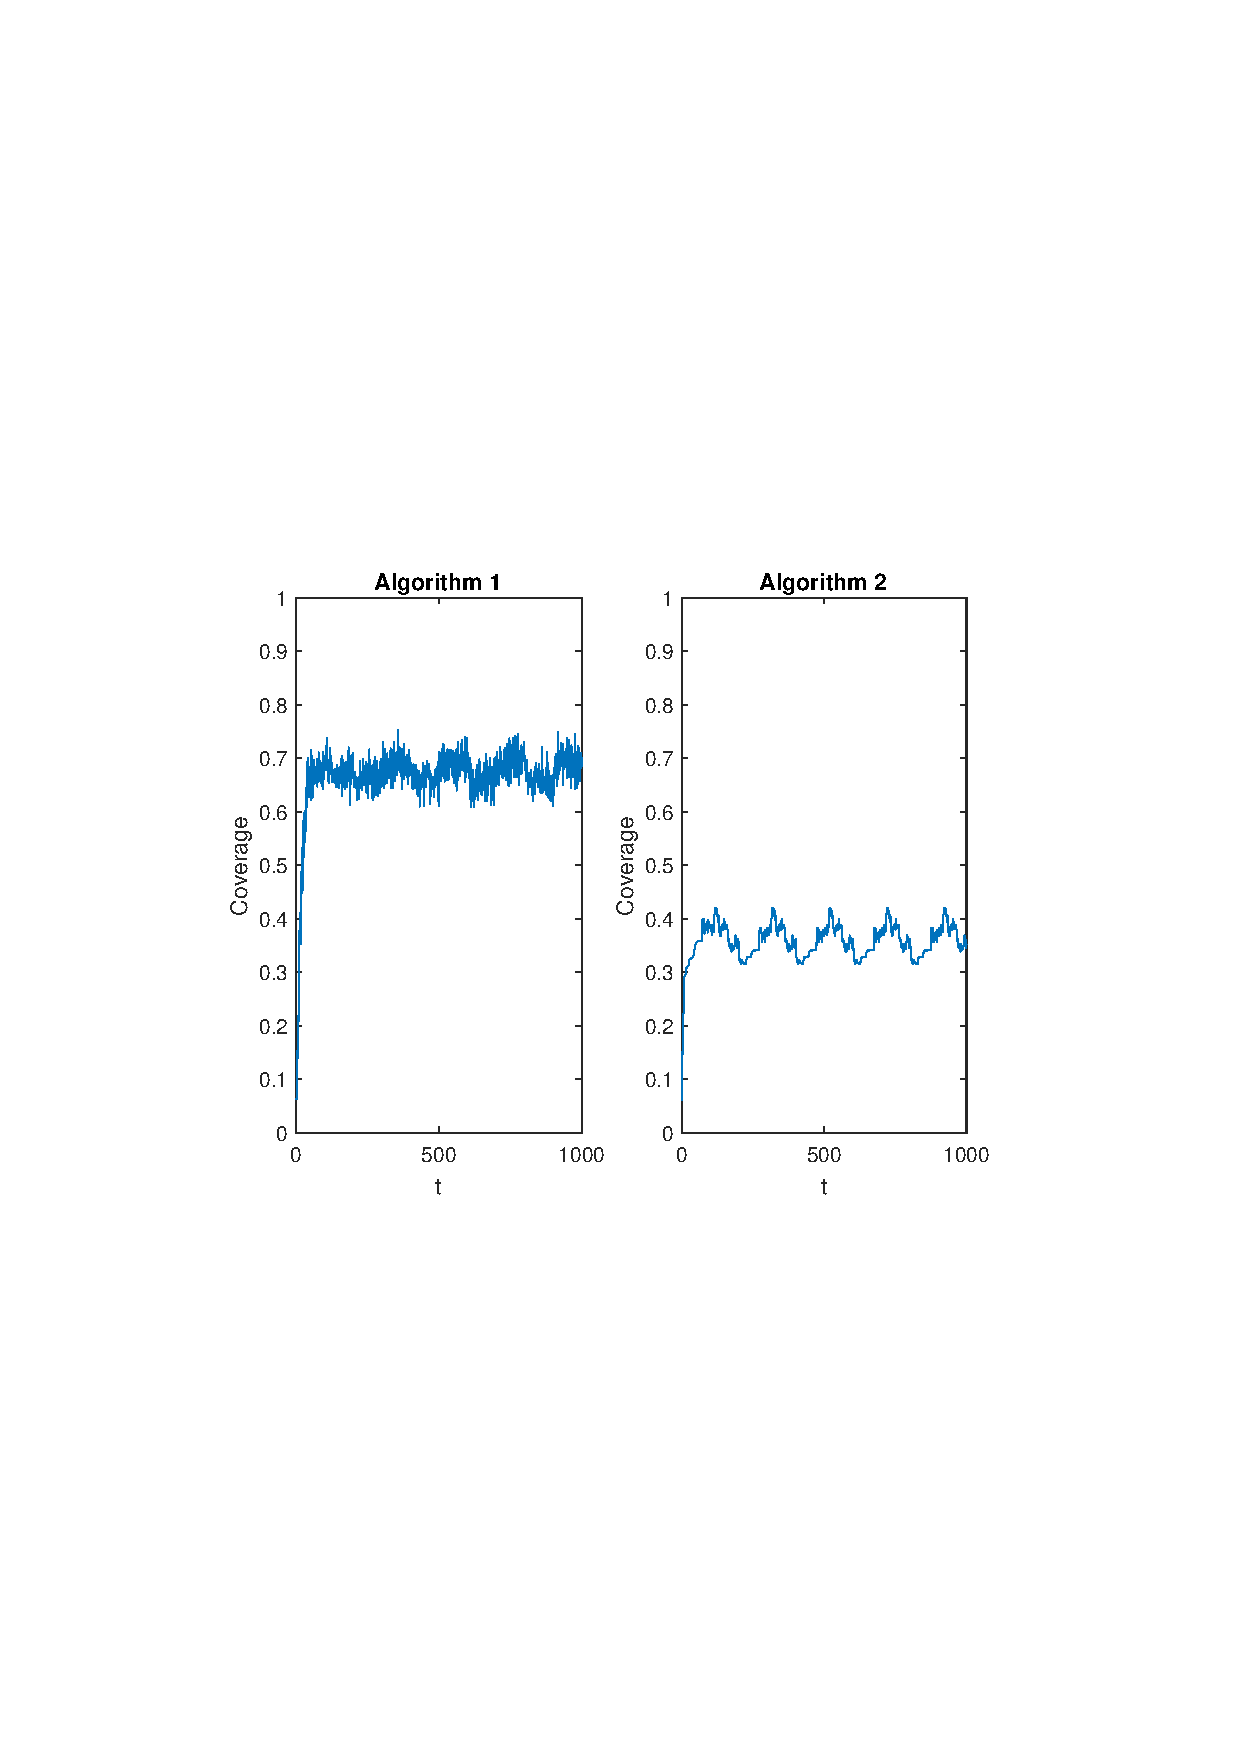
\includegraphics[scale=0.7, trim={3cm 10cm 4cm 9cm},clip]{graphics/coverage_alg1_vs_alg2_1000steps_LIFETIME200.pdf}
\caption{Algorithm 1 vs. Algorithm 2 in 1000 steps with lifetime 200}
\label{fig:alg1vsalg2_200}
\end{figure}

Algorithm 1 also does a better job of maintaining the coverage while repopulating the system, but that can be seen in Figure \ref{fig:alg1vsalg2_200}. Each 200 steps a balloon is removed, and recreated at coordinates (0,0). Like mentioned earlier, Algorithm 1 does any excellent job of spreading the balloons quickly and thoroughly so this lifetime heavily favours that algorithm. Algorithm 2 is never able to spread the balloons well enough before it has to start all over again.


\subsection{Algorithm 3}
The third algorithm is a modification of the second algorithm and introduces a new feature to the balloon. The second algorithm based its decision on the number of balloons in the neighbouring cells, and which wind layer would blow it to the most vacant cell. 

The third algorithm communicates with the balloons in its communication radius and makes the decision based on the data it receives. This is done through a private function. The function creates a list of all balloons within the communication radius. Then each of the balloons in that list counts it own neighbours and returns the value. The balloon with the fewest number of neighbours is deemed as a critical point. 

\begin{figure}[H]
    \centering
    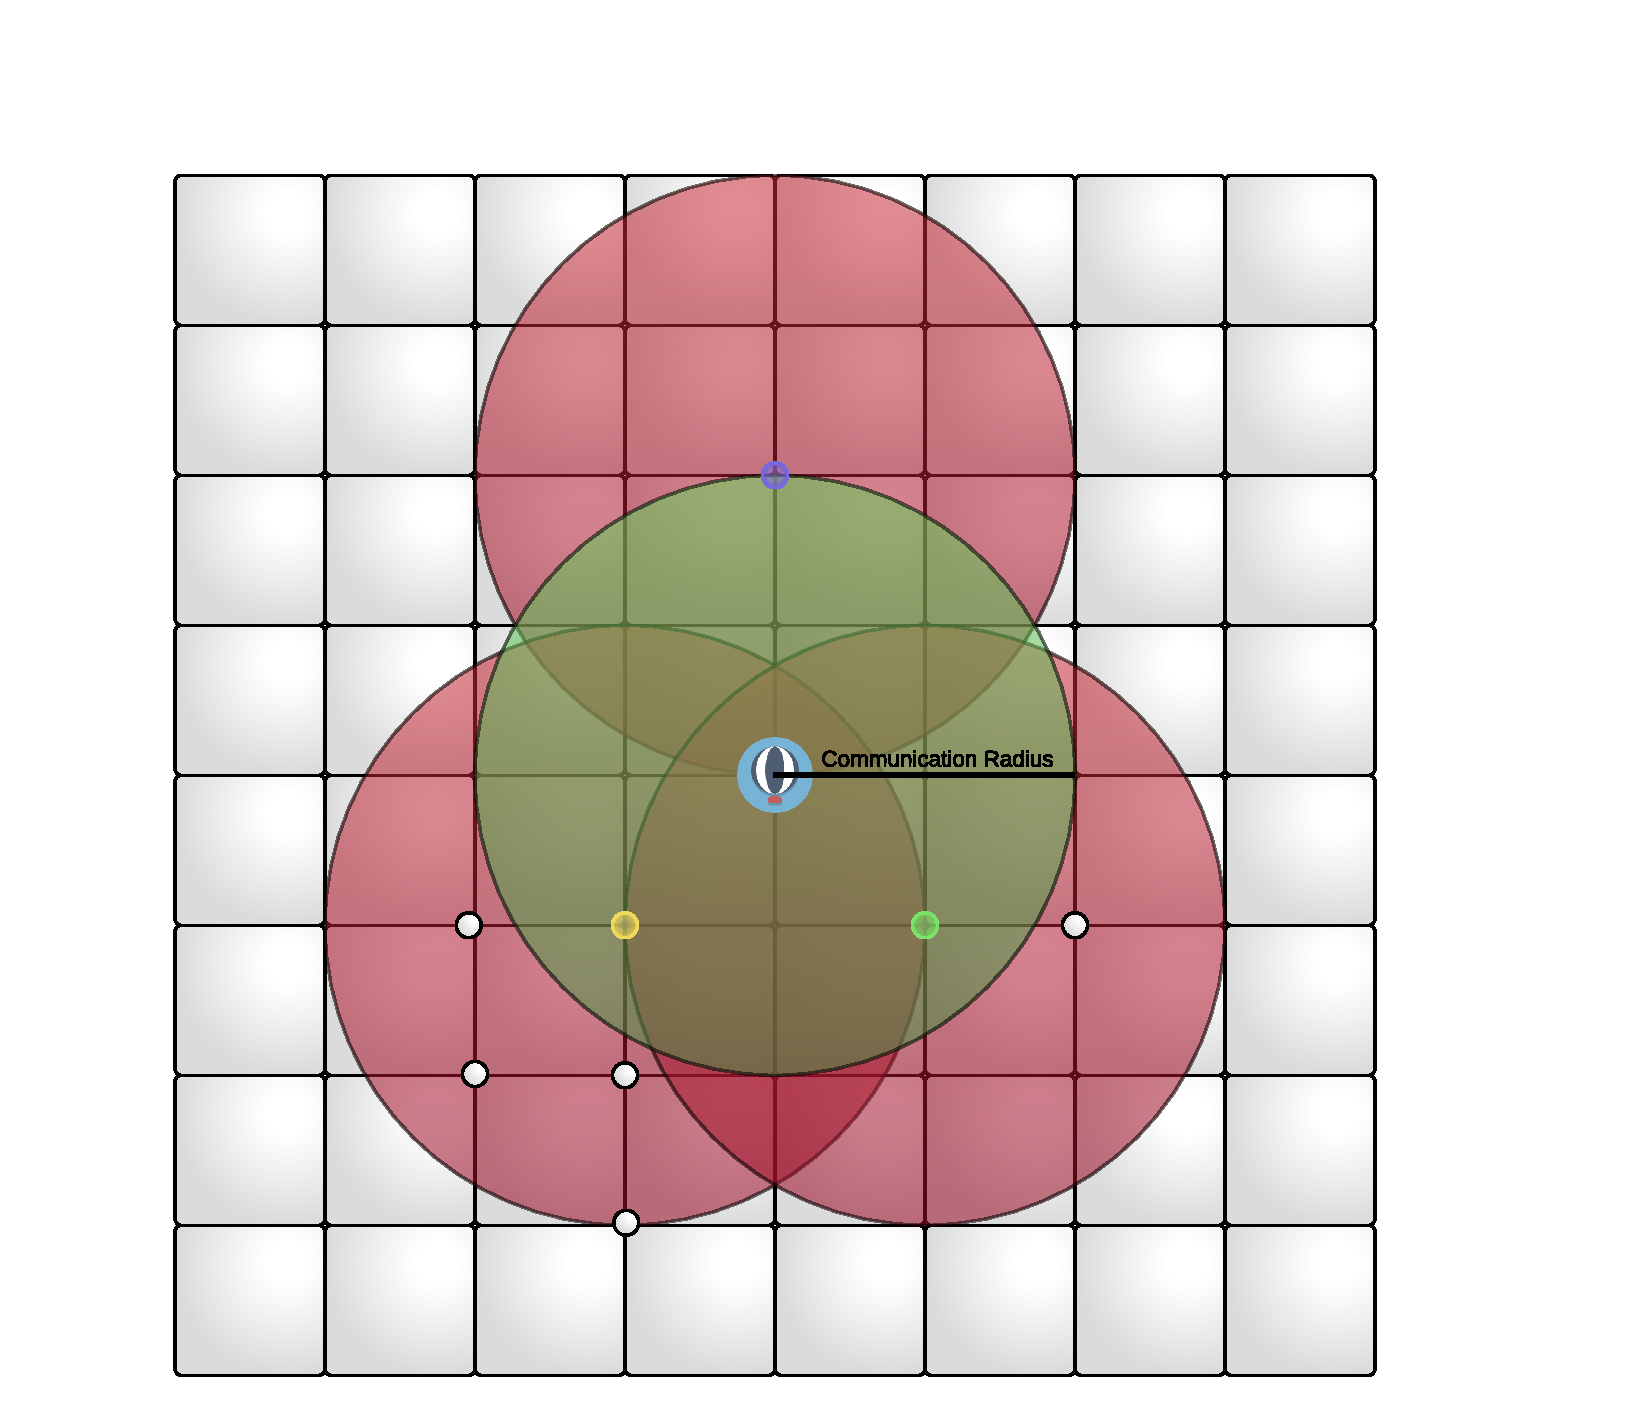
\includegraphics[scale=0.5]{graphics/criticalPointimproved.pdf}
    \caption{Critical point computed. The blue point will be deemed critical}
    \label{fig:criticalf}
\end{figure}

Figure \ref{fig:criticalf} shows an example of calculations of a critical point. The main balloon has three neighbours represented with different colours. Each of the three neighbours has its own number of neighbours. The yellow, green and purple balloons each have 6, 3 and 1 neighbours respectively. This means that the coordinates of the purple balloon are returned as a critical point.

Algorithm 3 is also the first algorithm to explore more than just the windlayer above and below, but the entire stratosphere. To be able to navigate towards that layer, a  \textit{nextLayer} attribute has been introduced to the balloon object. When a balloon is moved between layers, this variable is used to determine if the vertical movement should be stopped or not, i.e if the balloon has reached is destined layer or not.

\begin{algorithm}[H]
  \If{More than 1 balloon at current space}{
  Find point c (critical point)\\
  
    Calculate projectedPair (pp) for current layer\\
    
    smallestPP = distance(pp, c)\\
  \ForAll{WindLayer wl : stratosphere} {
  
  Calculate projectedPair (pp) 
  
  Calculate distance(pp,c)
  
  \If{pp$<$smallestPP}{wl is chosen as NextLayer}}
  \EndFor
  
  NextLayer set as attribute of balloon
  
\If{NextLayer is above CurrentLayer}{
goUp()
}
\Else{
goDown()
}

 }
 \Else
 {Stay in current layer}
 \caption{Control Algorithm 3}
 \label{alg3}
\end{algorithm}

\begin{figure}
    \centering
    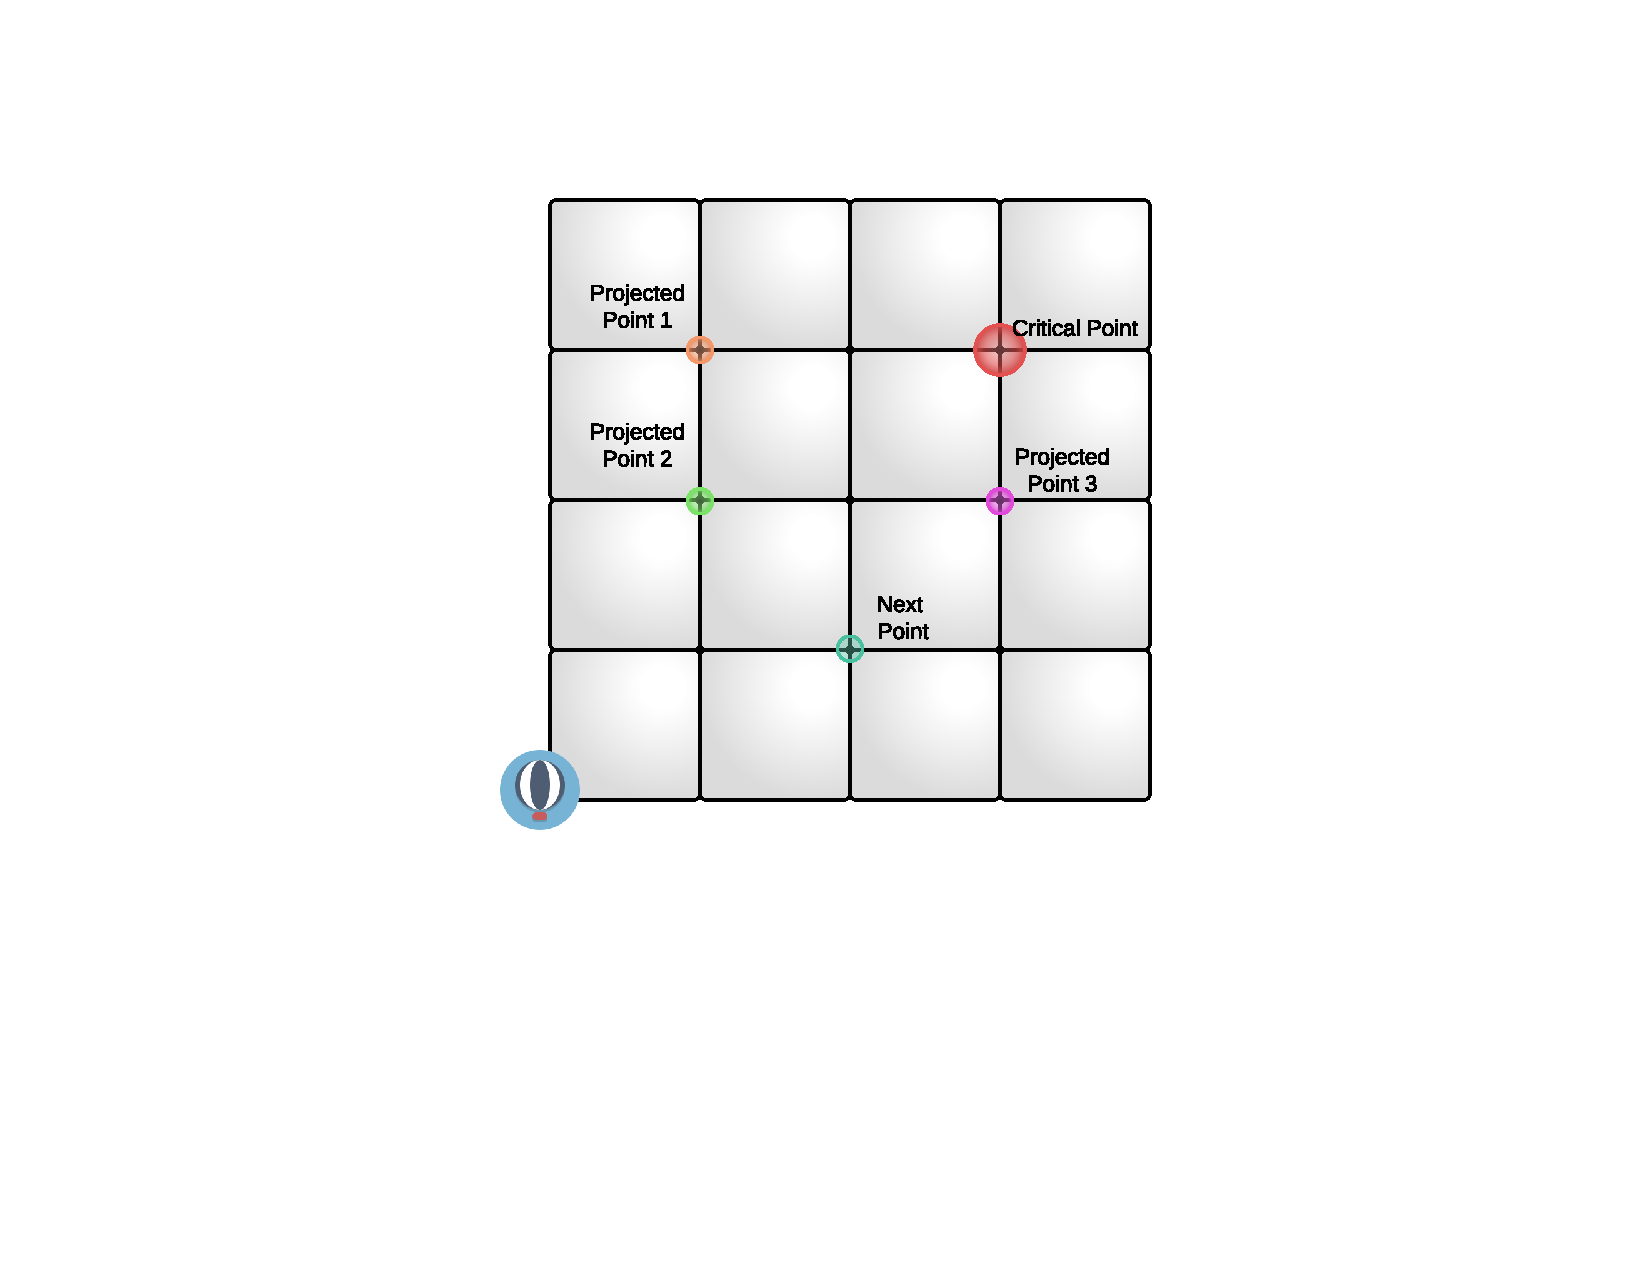
\includegraphics[width=\textwidth, trim=5cm 7cm 5cm 3.3cm, clip]{graphics/projectedPoints.pdf}
    \caption{Critical point computed}
    \label{fig:critical}
\end{figure}

When a critical point has been determined, a projection point is created for all wind layers in the stratosphere. This is represented in figure \ref{fig:critical}. The distance $d$ between each projection point ($x_p, y_p$) and the critical point ($x_c,y_c$) is calculated with the following formula:

\begin{align}
d = \sqrt{(x_c-x_p)^2+(y_c-y_p)^2} \notag
\end{align}

\subsection{Algorithm 3s}
Algorithm 3 was the first algorithm to offer movement between multiple layers at a time. The transition does not happen instantaneously since a balloon has a fixed vertical speed. This means that a balloon can be interrupted in its transition, and the destination layer changed before the balloon reaches its target. Algorithm 3s is a minor twist on Algorithm 3 as it only adds one criteria. No decision is made by balloons that are already in motion:

\begin{algorithm}[H]
\ForAll{Ballon b : balloons}{
\If{b is not moving vertically}{applyDecision3(b)}
}
\caption{Control Algorithm 3s}
\label{alg:3s}
\end{algorithm}

Figures \ref{fig:alg3vsalg3s_long} and \ref{fig:alg3vsalg3s_200} show the performance of the algorithms, first with an infinite lifetime of all balloons. There the coverage is fairly similar once the simulation has created all balloons. The second simulation is with lifetime of 200 steps. Algorithm 3 does a decent job of keeping stable, while the coverage with Algorithm 3s plunges every 200 steps in the simulation. With this extra criteria in place it makes the algorithm slower to respond to changes since each balloon does not respond while it is currently undertaking a change in altitude. The conclusion is that 

\begin{figure}
\centering
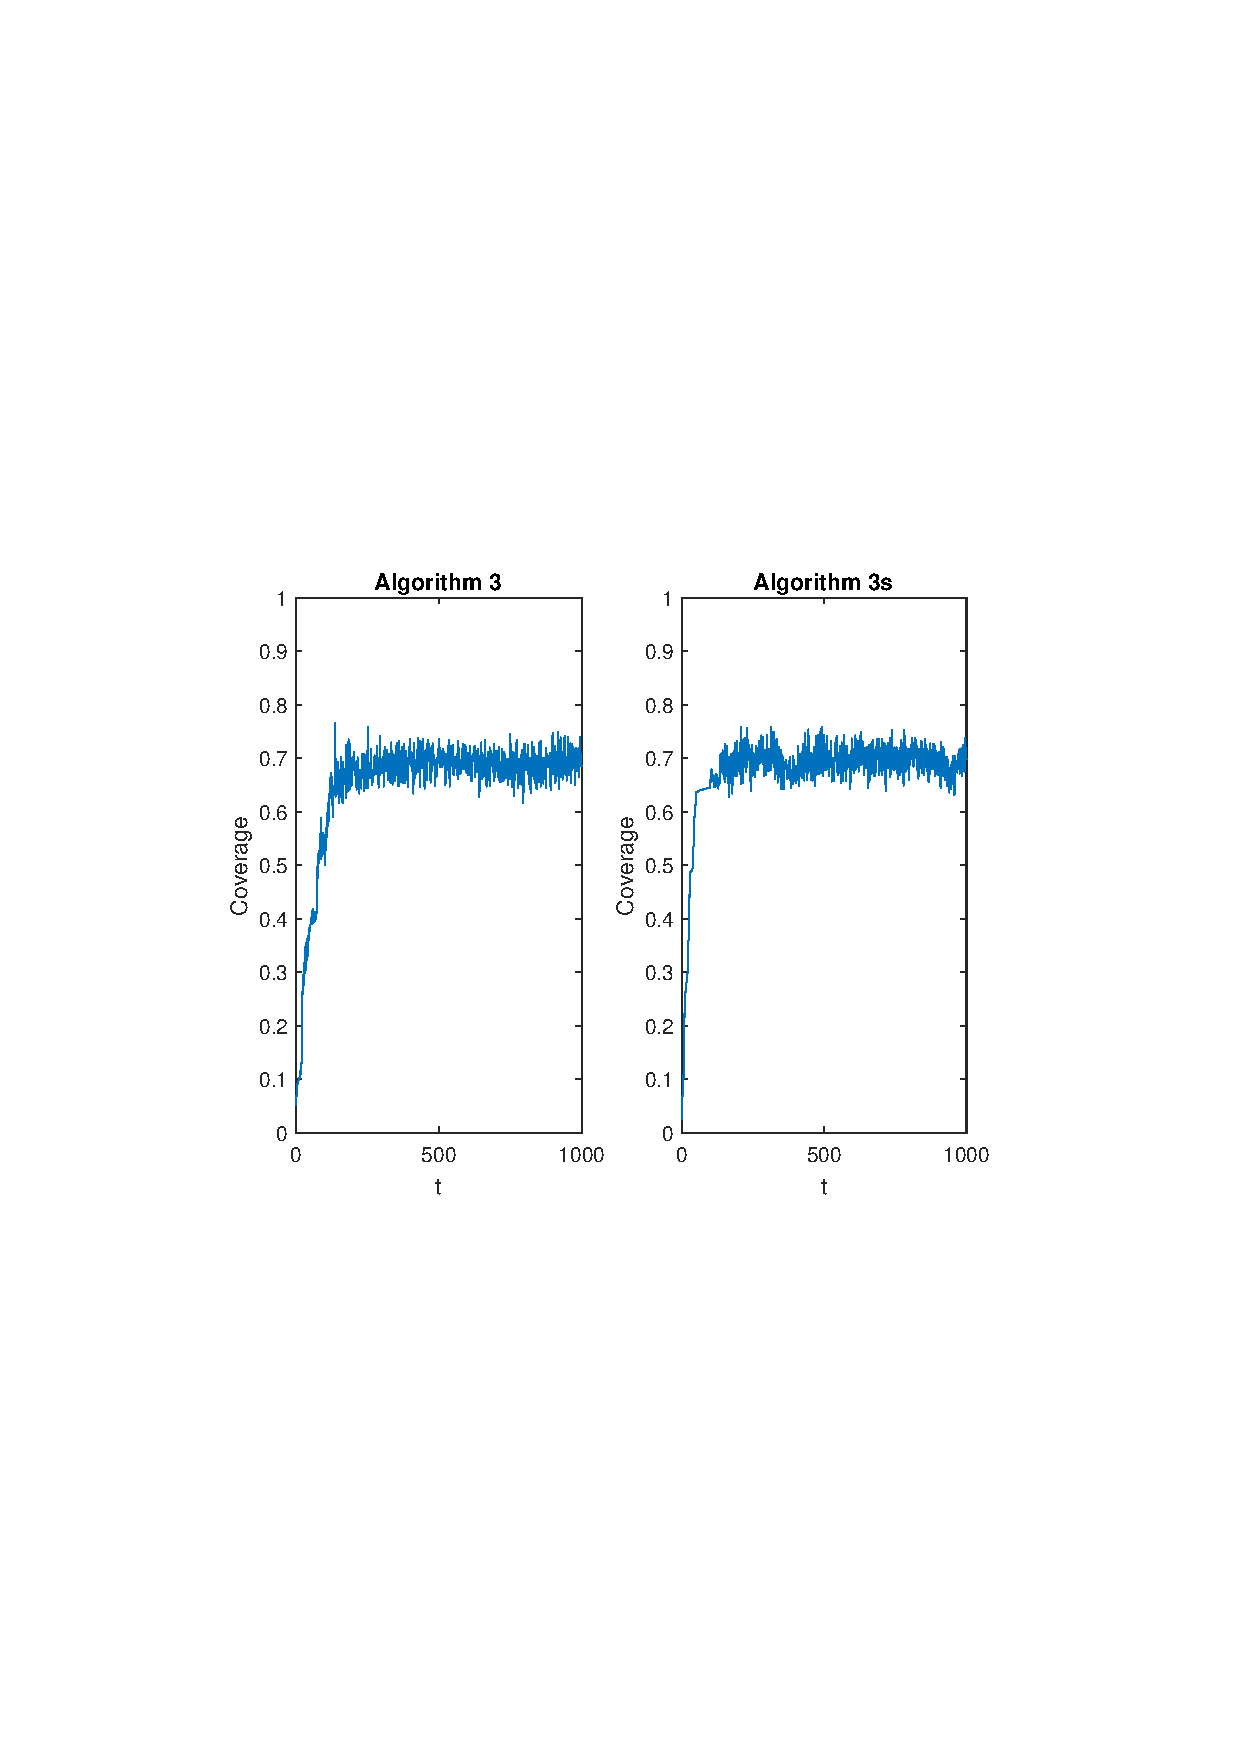
\includegraphics[scale=0.7, trim={3cm 10cm 4cm 9cm},clip]{graphics/coverage_alg3_vs_alg3s_1000steps_LIFETIMELONG.pdf}
\caption{Algorithm 3 vs. Algorithm 3s in 1000 steps with an infinite lifetime of each balloon }
\label{fig:alg3vsalg3s_long}
\end{figure}
\begin{figure}
\centering
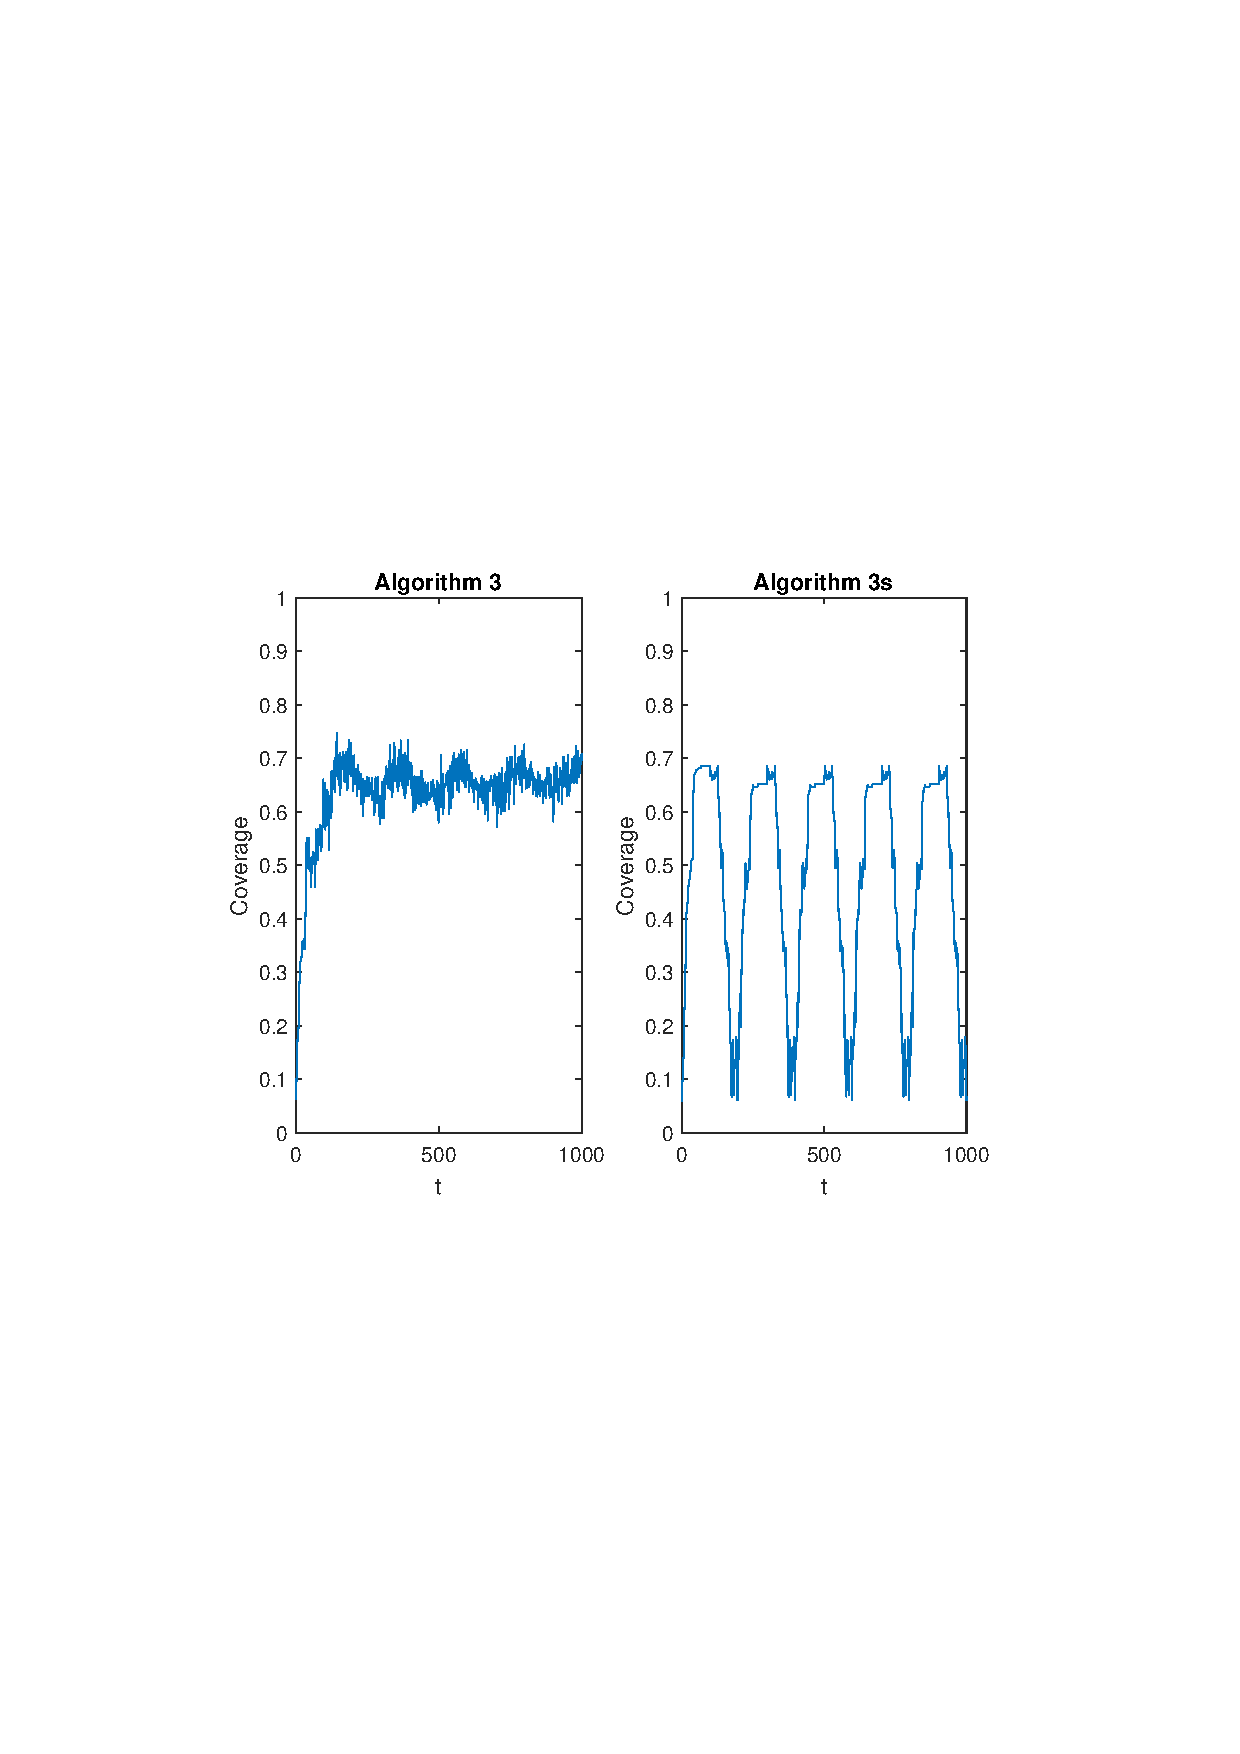
\includegraphics[scale=0.7, trim={3cm 10cm 4cm 9cm},clip]{graphics/coverage_alg3_vs_alg3s_1000steps_LIFETIME200.pdf}
\caption{Algorithm 3 vs. Algorithm 3s in 1000 steps with lifetime 200}
\label{fig:alg3vsalg3s_200}
\end{figure}


\subsection{Algorithm 4}
How does a balloon know the wind direction and speed in its neighbouring wind layers? How does a balloon that has drifted several hundred kilometers from the others determine which direction to take? The most realistic way of determining what the weather conditions are like in another layer, is by communicating with a balloon currently locating in said layer. This is what Algorithm 4 introduces. 

This approach is more realistic and accurate as it can provide the balloons with live weather data. The model is however still constructed with static wind data which is initialized when the class is created and never updated. But the access, and the way in which balloons acquire data for their decision is changed as of Algorithm 4. This method does however have an obvious pitfall. Since all balloons are launched in the same wind layer, no one will ever know the condition in other wind layers and therefore stay put. This problem is circumvented with a quick fix: Algorithm 1. Since that algorithm did such an excellent job of spreading the balloons on the initial stages it is utilized here in Algorithm 4.

\begin{algorithm}[H]
\ForAll{Balloon b : balloons}{
\If{b.age $<$ 50}{applyDecision1(b)}{}
\Else{
ArrayList n = find all neighbours\\

ArrayList w = extract wind layers from n \\

Find critical point \\

Choose wind layer (from w) that directs towards it
}
}
\caption{Control Algorithm 4}
\label{alg:4}
\end{algorithm}

When the age of a balloon has reached 50 (randomly chosen) the logic is the same as Algorithm 3, but with more limited resources. Algorithm 3 had access to all layers in the system, while Algorithm 4 has to depend on the position of its neighbours. This method clearly favours herding since staying close to the pack gives a balloon more data to work from. But the logic however always tries to steer the balloon away from the most crowded areas. 

\begin{figure}
\centering
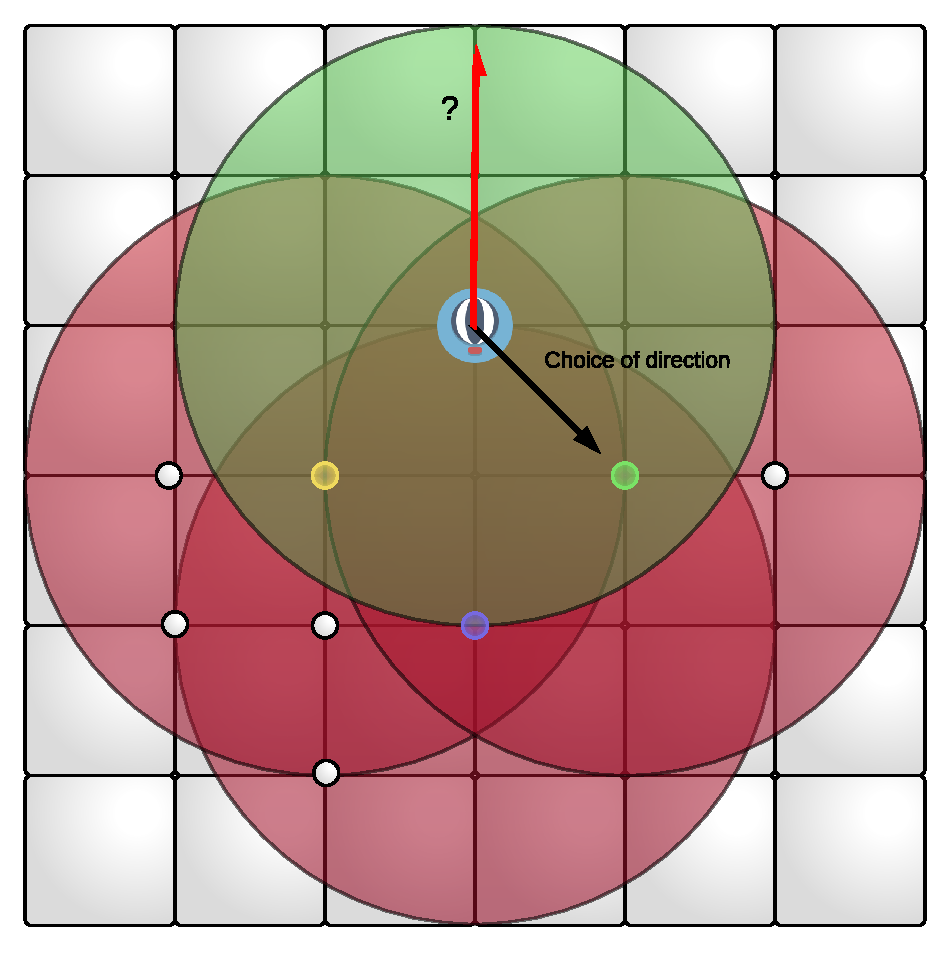
\includegraphics[scale = 0.3]{graphics/errorWithLogicCritical.pdf}
\caption{The problem is that the algorithm moves to the least occupied area, but not the empty area}
\label{fig:errorLogic}
\end{figure}

The flaw with the logic of Algorithm 3 and 4 is displayed in Figure \ref{fig:errorLogic}. As the balloon does not have access to every point on the grid, it makes its decision based on the neighbouring balloons. This means that the balloon will always navigate towards another balloon. This is a flaw when it comes to spreading, but an advantage as the balloons always need to be in contact with each other. 

\subsection{Algorithm 4s}
\begin{figure}
\centering
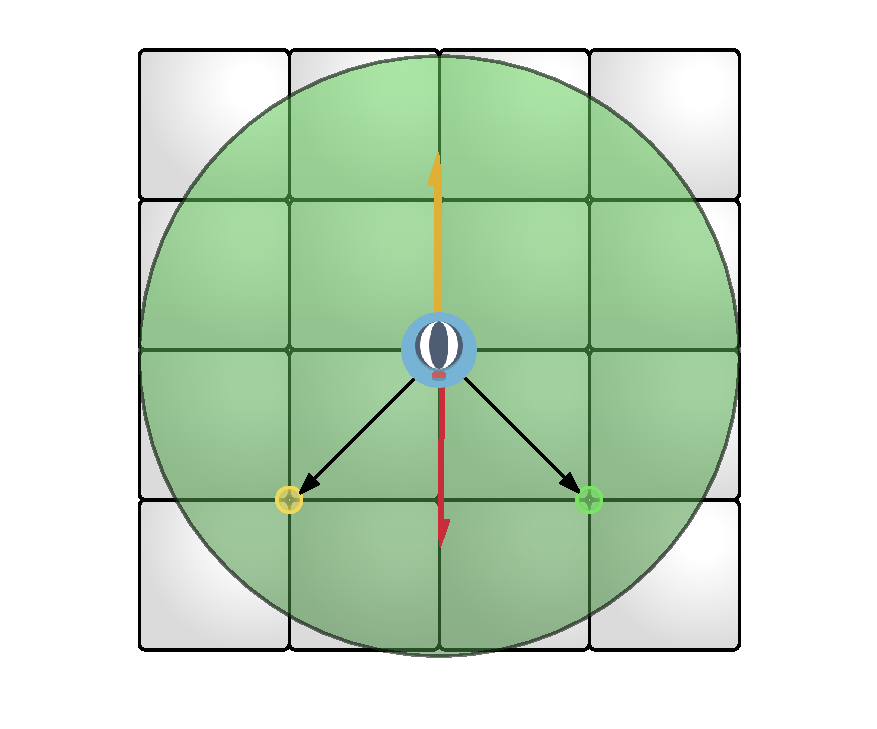
\includegraphics[scale = 0.3]{graphics/alg4s.pdf}
\caption{Algorithm 4s moves against all crowds}
\label{fig:alg4s}
\end{figure}

Like the $s$ suggests, Algorithm 4s is minor tweak of Algorithm 4. Like displayed in Figure \ref{fig:alg4s} this algorithm focuses on moving balloons away from all of their neighbours. This is done by adding the direction vectors from the balloon to each of the neighbours together, and computing the vector that points to the opposite direction. The movement to that particular direction is however still dependent on only the wind layers found in the neighbourhood. The balloon can still not choose perfectly its direction, but rather chooses between from a limited selection of wind layers.

\begin{algorithm}[H]
\ForAll{Balloon b : balloons}{
\If{b.age $<$ 50}{applyDecision1(b)}{}
\Else{
ArrayList n = find all neighbours\\

ArrayList w = all wind layers from n and b\\

Compute vector r (Red vector on figure \ref{fig:alg4s})\\

Create vector y (Yellow vector on figure \ref{fig:alg4s} )\\

Choose layer from w with direction closest to y. 
}}
\caption{Control Algorithm 4s}
\label{alg:4s}
\end{algorithm}


\begin{figure}[H]
\centering
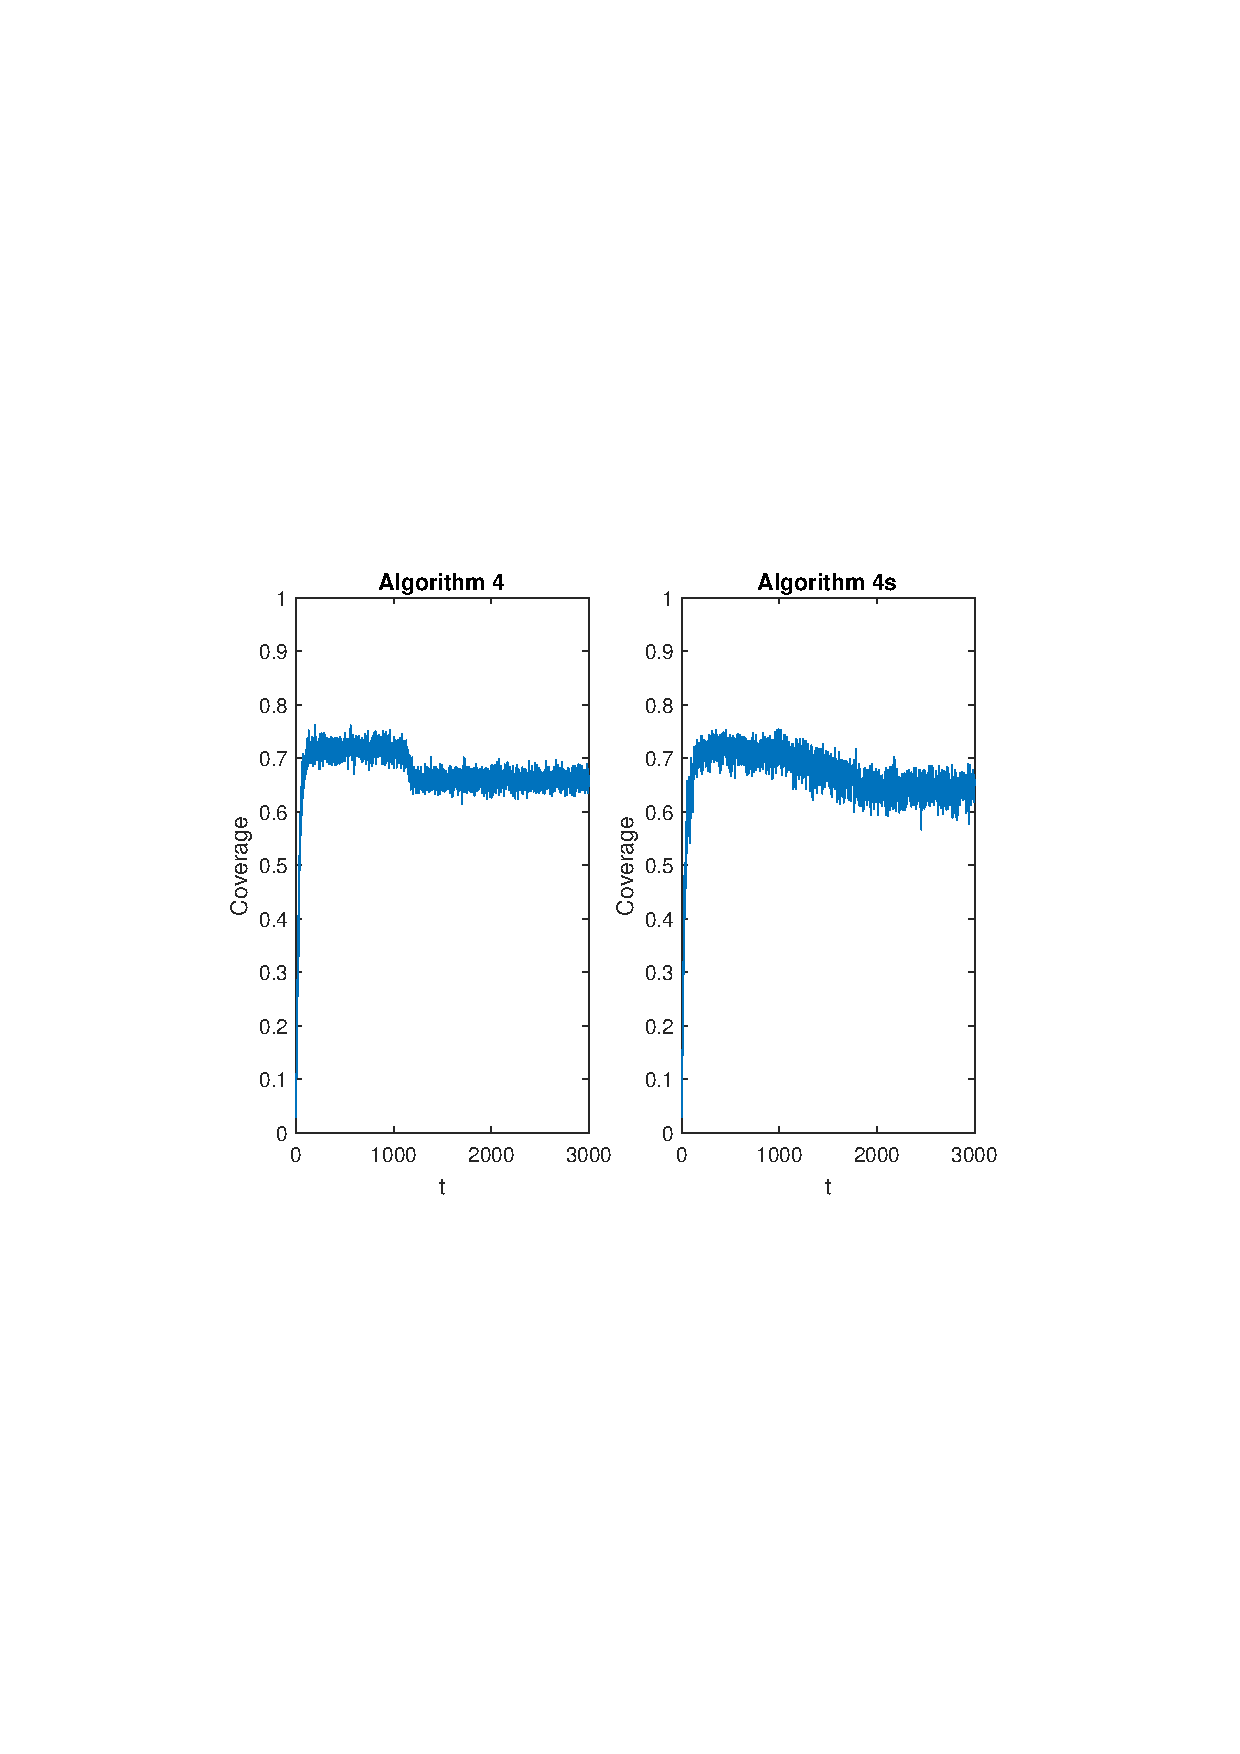
\includegraphics[scale=0.7, trim={3cm 10cm 4cm 9cm},clip]{graphics/coverage_alg4_vs_alg4s_3000_LONG.pdf}
\caption{Algorithm 4 vs. Algorithm 4s in 3000 steps with an infinite lifetime of each balloon}
\label{fig:alg4vsalg4s_long}
\end{figure}

\begin{figure}[H]
\centering
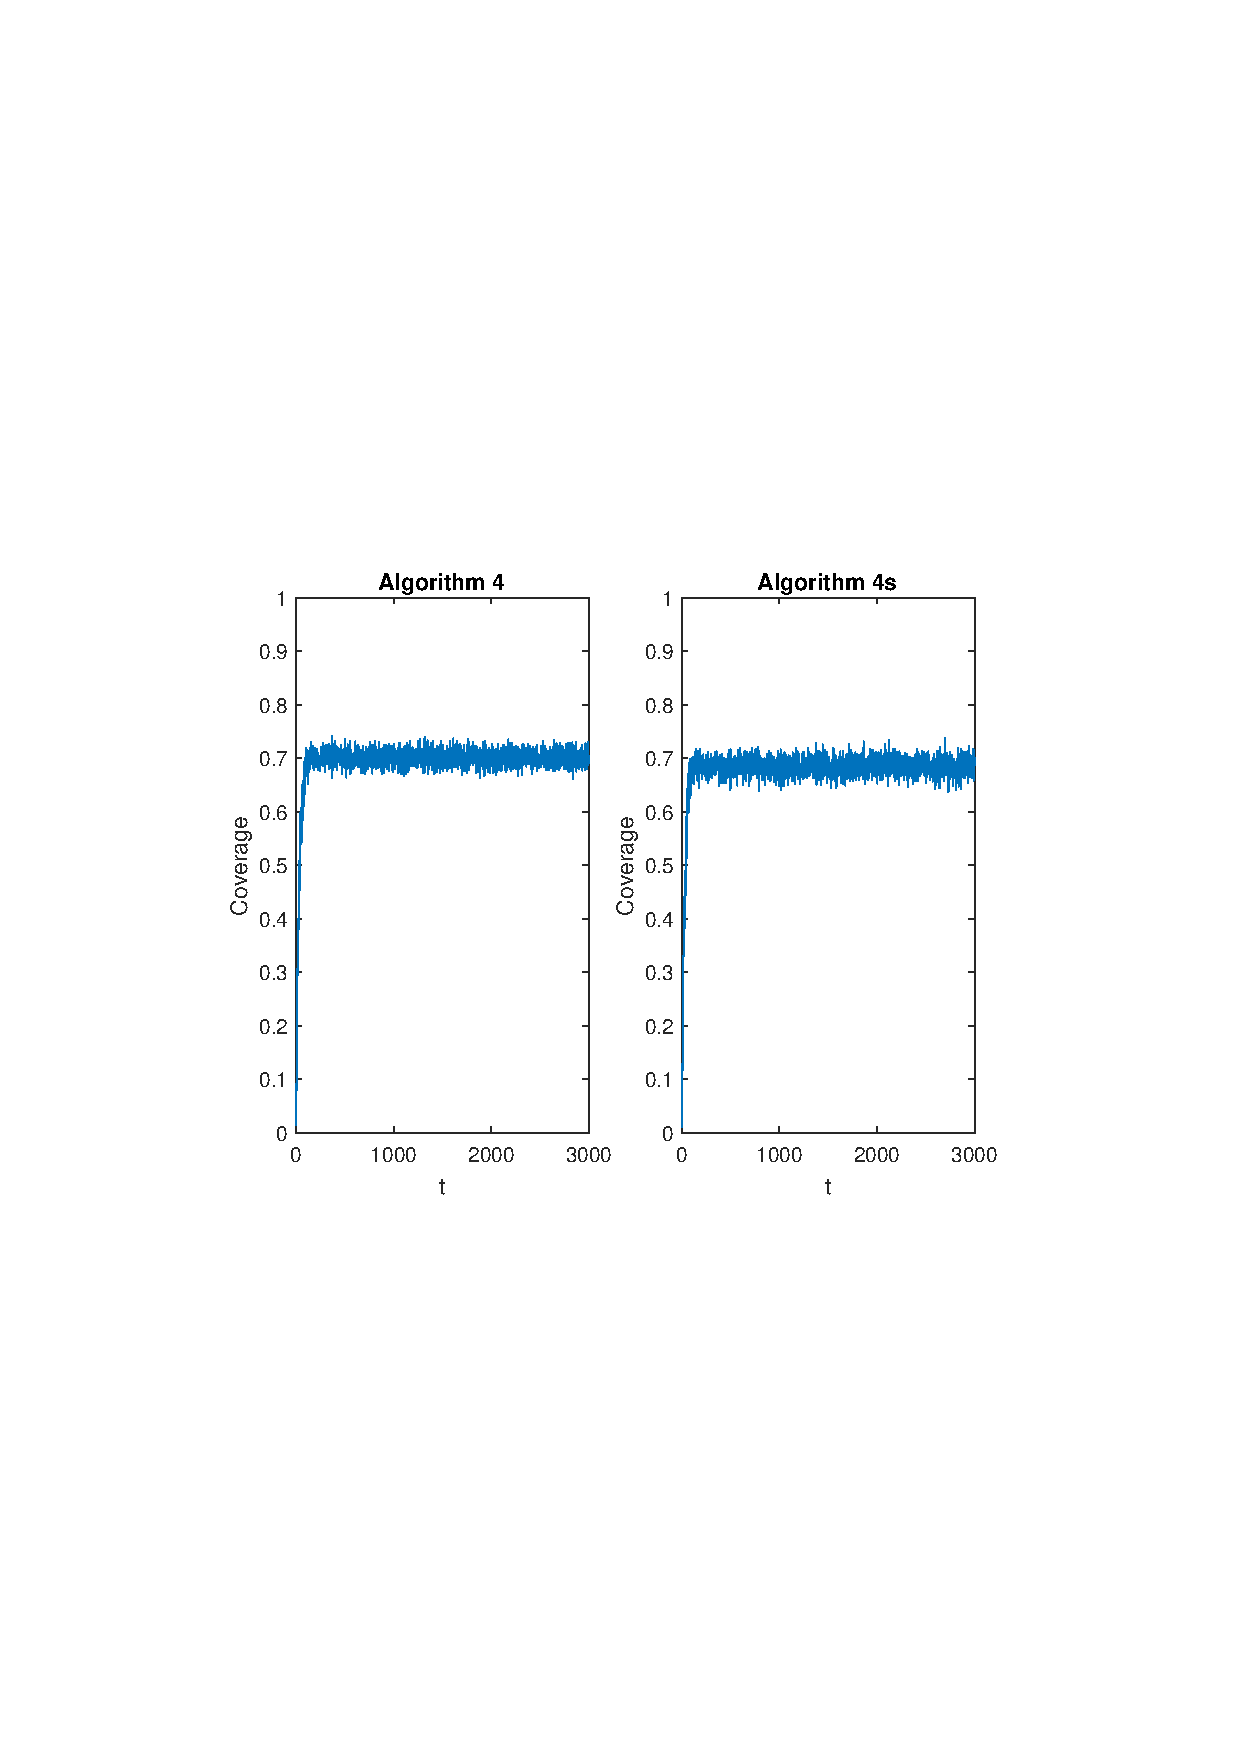
\includegraphics[scale=0.7, trim={3cm 10cm 4cm 9cm},clip]{graphics/coverage_alg4_vs_alg4s_3000_200.pdf}
\caption{Algorithm 4 vs. Algorithm 4s in 3000 steps with lifetime 200}
\label{fig:alg4vsalg4s_200}
\end{figure}

It is interesting to see that both Algorithm 4 and 4s both perform better when the balloon has a fixed lifetime. The coverage is stable and relatively similar. 

\begin{table}[]
\centering

\begin{tabular}{r|l|l|}

\textbf{Statistic}                 & \textbf{Algorithm 4} & \textbf{Algorithm 4s} \\ \hline
\textbf{Runtime (ms):}                  & 12610             & 9427                  \\ \hline
\textbf{Coverage over simulation:} & 69.5\%               & 67.9 \%               \\ \hline
\textbf{Dropped Connections:}      & 826.054              & 902.472               \\ \hline
\end{tabular}
\caption{Results. Algorithm 4 vs. 4s}
\label{tbl:res}
\end{table}

Table \ref{tbl:res} shows better the difference between the two, but Algorithm 4 has just slightly better coverage and more stable as well as it loses fewer connections during the simulation.



\section{Discussion}
This project is like Pandora's box. The idea is so simple and conceivable and creating a model for it sounds like a piece of cake. Circles floating around some area according to some predefined wind speed. But the considerations and details are endless. A long discussion could be had about each detail of the model but that is material for a whole other project. To keep things short and precise some key points have been chosen that are interesting to give a second thought to.
\subsection{Assumptions}
All of the assumptions can be discussed to great lengths and scrutinized, but that is the nature of assumptions.
\subsection{Decentralized vs. Centralized}
There are two ways to implement the control of the balloons. With a centralized algorithm or decentralized, each with its pros and cons. With a centralized solution every balloon must be in contact with the main data source at every given moment. This means that the balloons have to stay close together, and always in connection with a ground station that crunches the numbers and provides the balloons with a decision. The controlling could be more accurate with this method, but also prone to failures, since the balloons rely so heavily on the ground connection.

A decentralized version is on the other hand more forgiving when it comes to connection. Each balloon can survive a temporary blackout and pays attention only to the object within its detection range. The controlling however would be shortsighted and a balloon would not see the forest for the trees in some sense.

The optimal solution is a mixture of centralized and decentralized algorithm. When possible, balloons would be provided with updated status of the entire system; the location of other balloons in the system and updated weather data. This would give the balloons capability to navigate without connection to the ground, but also a frequent overview of the system as a whole. 
\subsection{Access to Data}
\subsection{Further Work}


\section{Conclusion}
%\input{}

\section{Questions (notes K\'ari)}
\begin{enumerate}
    \item Is the model centralized or decentralized? Centralized
    \item What are the pros and cons of centralized vs. decentralized?
    \item How do I add my own control algorithm to the model?
    \item Why does the decision happen before the move function? Does it matter?
    \item How do I supply the model with my own wind data?
    \item How do I add more than 4 layers?
\end{enumerate}




\pagebreak
\printnomenclature
\nocite{*}
\bibliography{library.bib}{} 
\bibliographystyle{apacite}

\end{document}